% Options for packages loaded elsewhere
\PassOptionsToPackage{unicode}{hyperref}
\PassOptionsToPackage{hyphens}{url}
\PassOptionsToPackage{dvipsnames,svgnames,x11names}{xcolor}
%
\documentclass[
]{article}
\usepackage{amsmath,amssymb}
\usepackage{lmodern}
\usepackage{iftex}
\ifPDFTeX
  \usepackage[T1]{fontenc}
  \usepackage[utf8]{inputenc}
  \usepackage{textcomp} % provide euro and other symbols
\else % if luatex or xetex
  \usepackage{unicode-math}
  \defaultfontfeatures{Scale=MatchLowercase}
  \defaultfontfeatures[\rmfamily]{Ligatures=TeX,Scale=1}
\fi
% Use upquote if available, for straight quotes in verbatim environments
\IfFileExists{upquote.sty}{\usepackage{upquote}}{}
\IfFileExists{microtype.sty}{% use microtype if available
  \usepackage[]{microtype}
  \UseMicrotypeSet[protrusion]{basicmath} % disable protrusion for tt fonts
}{}
\makeatletter
\@ifundefined{KOMAClassName}{% if non-KOMA class
  \IfFileExists{parskip.sty}{%
    \usepackage{parskip}
  }{% else
    \setlength{\parindent}{0pt}
    \setlength{\parskip}{6pt plus 2pt minus 1pt}}
}{% if KOMA class
  \KOMAoptions{parskip=half}}
\makeatother
\usepackage{xcolor}
\usepackage[margin=1in]{geometry}
\usepackage{graphicx}
\makeatletter
\def\maxwidth{\ifdim\Gin@nat@width>\linewidth\linewidth\else\Gin@nat@width\fi}
\def\maxheight{\ifdim\Gin@nat@height>\textheight\textheight\else\Gin@nat@height\fi}
\makeatother
% Scale images if necessary, so that they will not overflow the page
% margins by default, and it is still possible to overwrite the defaults
% using explicit options in \includegraphics[width, height, ...]{}
\setkeys{Gin}{width=\maxwidth,height=\maxheight,keepaspectratio}
% Set default figure placement to htbp
\makeatletter
\def\fps@figure{htbp}
\makeatother
\setlength{\emergencystretch}{3em} % prevent overfull lines
\providecommand{\tightlist}{%
  \setlength{\itemsep}{0pt}\setlength{\parskip}{0pt}}
\setcounter{secnumdepth}{-\maxdimen} % remove section numbering
\newlength{\cslhangindent}
\setlength{\cslhangindent}{1.5em}
\newlength{\csllabelwidth}
\setlength{\csllabelwidth}{3em}
\newlength{\cslentryspacingunit} % times entry-spacing
\setlength{\cslentryspacingunit}{\parskip}
\newenvironment{CSLReferences}[2] % #1 hanging-ident, #2 entry spacing
 {% don't indent paragraphs
  \setlength{\parindent}{0pt}
  % turn on hanging indent if param 1 is 1
  \ifodd #1
  \let\oldpar\par
  \def\par{\hangindent=\cslhangindent\oldpar}
  \fi
  % set entry spacing
  \setlength{\parskip}{#2\cslentryspacingunit}
 }%
 {}
\usepackage{calc}
\newcommand{\CSLBlock}[1]{#1\hfill\break}
\newcommand{\CSLLeftMargin}[1]{\parbox[t]{\csllabelwidth}{#1}}
\newcommand{\CSLRightInline}[1]{\parbox[t]{\linewidth - \csllabelwidth}{#1}\break}
\newcommand{\CSLIndent}[1]{\hspace{\cslhangindent}#1}
\usepackage{booktabs}
\usepackage{longtable}
\usepackage{array}
\usepackage{multirow}
\usepackage{wrapfig}
\usepackage{float}
\usepackage{colortbl}
\usepackage{pdflscape}
\usepackage{tabu}
\usepackage{threeparttable}
\usepackage{threeparttablex}
\usepackage[normalem]{ulem}
\usepackage{makecell}
\usepackage{xcolor}
\usepackage{fontspec}
\usepackage{multicol}
\usepackage{hhline}
\newlength\Oldarrayrulewidth
\newlength\Oldtabcolsep
\usepackage{hyperref}
\ifLuaTeX
  \usepackage{selnolig}  % disable illegal ligatures
\fi
\IfFileExists{bookmark.sty}{\usepackage{bookmark}}{\usepackage{hyperref}}
\IfFileExists{xurl.sty}{\usepackage{xurl}}{} % add URL line breaks if available
\urlstyle{same} % disable monospaced font for URLs
\hypersetup{
  pdftitle={Disentangling the spinal mechanisms of illusory heat and burning sensations in the Thermal Grill Illusion},
  pdfauthor={Alexandra G. Mitchell1, Jesper Fischer Ehmsen1, Daniel Elmstrom Christensen1, Anna Villaume Stuckert2, Patrick Haggard3, Francesca Fardo1,4},
  colorlinks=true,
  linkcolor={blue},
  filecolor={Maroon},
  citecolor={Blue},
  urlcolor={Blue},
  pdfcreator={LaTeX via pandoc}}

\title{Disentangling the spinal mechanisms of illusory heat and burning
sensations in the Thermal Grill Illusion}
\author{Alexandra G. Mitchell\textsuperscript{1}, Jesper Fischer
Ehmsen\textsuperscript{1}, Daniel Elmstrom
Christensen\textsuperscript{1}, Anna Villaume
Stuckert\textsuperscript{2}, Patrick Haggard\textsuperscript{3},
Francesca Fardo\textsuperscript{1,4}}
\date{}

\begin{document}
\maketitle

\textsuperscript{1}Center of Functionally Integrative Neuroscience,
Department of Clinical Medicine, Aarhus University, Denmark

\textsuperscript{2}Department of Neuroscience, Copenhagen University,
Denmark

\textsuperscript{3}Institute of Cognitive Neuroscience, University
College London, United Kingdom

\textsuperscript{4}Danish Pain Research Center, Department of Clinical
Medicine, Aarhus University, Denmark

Corresponding authors: Alexandra G. Mitchell
(\href{mailto:agmitchell@cfin.au.dk}{\nolinkurl{agmitchell@cfin.au.dk}})
and Francesca Fardo
(\href{mailto:francesca@cfin.au.dk}{\nolinkurl{francesca@cfin.au.dk}})

\hypertarget{abstract}{%
\section{Abstract}\label{abstract}}

The Thermal Grill Illusion (TGI) is a phenomenon in which the
juxtaposition of innocuous warm and cold temperatures elicits a burning
sensation, offering a unique window to understand how pain can be
perceived in response to harmless stimuli. Much debate has revolved
around whether spinal mechanisms are involved in the generation of
illusory pain, beyond supraspinal mechanisms. In this study, we
investigated the role of the spinal cord in the generation of the TGI,
in two independent experiments, involving a total of 80 healthy
individuals. We applied heat and cold stimuli on dermatomes, namely
areas of skin innervated by a single spinal nerve, mapped onto adjacent
or nonadjacent spinal segments. Participants were asked to rate their
perceptions of cold, warm, and burning sensations in response to TGI and
control stimuli. Our aims were to investigate thermosensory and painful
perceptual components of the TGI, as well as spatial features of the
illusion that may illuminate processes underlying thermosensory
integration in the spinal cord. Our findings revealed that both
thermosensory and painful components of TGI perception were modulated
similarly, with enhanced warm and burning ratings observed when cold and
warm stimuli were confined within the same dermatome. Further, we found
no perceptual differences based on the proximal-distal location of the
cold stimulus within a single dermatome, but notable heat enhancement
when the cold rather than the warm stimulus was associated with a more
caudal segmental location along the spinal cord. These results provide
insights into the organisation of the spinal cord in relation to the
thermosensory integration and generation of the TGI.

\newpage

\hypertarget{introduction}{%
\section{Introduction}\label{introduction}}

The thermal grill illusion (TGI) is a perceptual phenomenon that
challenges conventional understanding of pain perception. It is a
sensation of burning heat or pain when harmless cold and warm
temperatures are applied to the skin simultaneously
(\protect\hyperlink{ref-craig_thermal_1994}{Craig and Bushnell 1994};
\protect\hyperlink{ref-craig_functional_1996}{Craig et al. 1996}).
Despite cold and warm temperatures being individually innocuous, their
combination produces a contradictory burning sensation, even so the
temperatures are insufficient to activate peripheral nociceptors. The
generation of this illusion is thus attributed to central nervous system
mechanisms (\protect\hyperlink{ref-craig_thermal_1994}{Craig and
Bushnell 1994}; \protect\hyperlink{ref-fardo_beyond_2020}{Fardo et al.
2020}). Recent studies have highlighted the involvement of the spinal
cord as an initial site contributing to the TGI
(\protect\hyperlink{ref-fardo_organization_2018}{Fardo, Finnerup, and
Haggard 2018}; \protect\hyperlink{ref-harper_conditioned_2017}{Harper
and Hollins 2017}). However, the precise mechanisms underpinning
integration of cold and warm thermal afferents in the spinal cord,
alongside those responsible for the distinctive burning quality to this
illusion, are yet to be elucidated.

The TGI is often described as encompassing two distinct perceptual
components - an illusion of heat and an illusion of pain Fardo et al.
(\protect\hyperlink{ref-fardo_beyond_2020}{2020}). The illusion of heat,
also known as synthetic heat
(\protect\hyperlink{ref-fruhstorfer_significance_2003}{Fruhstorfer,
Harju, and Lindblom 2003};
\protect\hyperlink{ref-green_localization_1977}{Green 1977},
\protect\hyperlink{ref-green_synthetic_2002}{2002},
\protect\hyperlink{ref-green_temperature_2004}{2004}), refers to
non-painful sensations evoked by the thermal grill
(\protect\hyperlink{ref-defrin_spatial_2008}{Defrin et al. 2008};
\protect\hyperlink{ref-kern_pharmacological_2008}{Kern et al. 2008};
\protect\hyperlink{ref-kern_effects_2008}{2008};
\protect\hyperlink{ref-bouhassira_investigation_2005}{Bouhassira et al.
2005}; \protect\hyperlink{ref-adam_relationships_2014}{Adam et al.
2014}). The illusion of pain, which is the most recognised aspect of the
TGI, is the distinctive burning sensation that accompanies the
simultaneous presentation of cold and warm stimuli
(\protect\hyperlink{ref-craig_thermal_1994}{Craig and Bushnell 1994};
\protect\hyperlink{ref-craig_functional_1996}{1996};
\protect\hyperlink{ref-bach_thermal_2011}{Bach et al. 2011}). The
hallmark of both illusory components is a qualitative change in
perception when the cold and warm stimuli are applied concurrently,
compared to when they are presented individually. Historically, the
thermosensory and painful components of the TGI were explained by
distinct spinal and supraspinal mechanisms, respectively. The enhanced
perception of heat in TGI was explained by a spinal inhibitory
mechanism, drawing from observations in an animal model where
simultaneous application of cold and warm temperatures reduced the
activity of cold-specific spinal neurons compared to when cold was
applied alone (\protect\hyperlink{ref-craig_thermal_1994}{Craig and
Bushnell 1994}). Instead, the illusory pain component was ascribed to a
disinhibition mechanism at the level of the thalamus, primarily based on
the observations of unremitting pain following thalamic lesions
(\protect\hyperlink{ref-craig_thermal_1994}{Craig and Bushnell 1994};
\protect\hyperlink{ref-craig_new_1998}{1998}).

Recent human studies on TGI provided differing interpretations of the
spinal or supraspinal origin of the illusion. Two studies posited that
the illusory pain component of the TGI depends uniquely on supraspinal
mechanisms. This interpretation was based on the observed modulation of
the illusion in accordance with a spatiotopic rather than somatotopic
representation of the body
(\protect\hyperlink{ref-marotta_transforming_2015}{Marotta, Ferrè, and
Haggard 2015}). Further, the illusion remained unaltered during
concomitant tactile stimulation, suggesting ineffectiveness of tactile
gating - a spinally-mediated process involving inhibition of nociceptive
activity by concurrent somatosensory activity
(\protect\hyperlink{ref-ferre_ineffectiveness_2018}{Ferrè et al. 2018}).
Counter to this perspective, other research endorsed a spinal
contribution to the TGI. These studies demonstrated that the illusion
varied depending on whether cold and warm stimuli were applied to
dermatomes mapped either onto adjacent or non-adjacent spinal segments
(\protect\hyperlink{ref-fardo_organization_2018}{Fardo, Finnerup, and
Haggard 2018}). Participants perceived the stimulation more veridically,
consistently with a reduction in TGI perception, when warm or cold
stimuli triggered more widespread activity along the spinal cord,
corroborating the hypothesis that the spinal cord is an initial site of
thermosensory integration underlying TGI. Further support for spinal
mechanisms comes from research demonstrating that both noxious heat and
the TGI were comparably reduced by conditioned pain modulation in
humans. This suggests a similar influence of descending modulation,
irrespective of whether the painful sensation was triggered by
potentially harmful (noxious) or harmless (innocuous) stimuli
(\protect\hyperlink{ref-harper_conditioned_2017}{Harper and Hollins
2017}). These findings collectively challenge a purely supraspinal
hypothesis of the painful component of the TGI and indicate the
relevance of spinal mechanisms in the manifestation of both illusory
heat and pain.

In this paper our objective was twofold. Firstly, we directly
investigated the hypothesis that thermosensory and burning components of
the TGI experience are mediated by spinal mechanisms in humans, by
manipulating the location of the stimuli within and across dermatomes.
Cold and warm stimuli were presented at a fixed distance on the skin,
but depending on their longitudinal or tangential orientation on the
arm, they elicited neural activity in a differing number of spinal
segments. Our assumption was that cold and warm-related neural activity
in the spinal cord was more focal, when the stimuli were presented
within the same dermatome, while more widespread, when the stimuli
mapped on non-adjacent spinal segments. Our past work using a similar
manipulation involved measuring the experience of the TGI using a
temperature matching task
(\protect\hyperlink{ref-fardo_organization_2018}{Fardo, Finnerup, and
Haggard 2018}), which provides a composite measure of TGI perception,
reflecting both thermosensory and painful components. Here, to probe
possible distinctions between the two qualitative components of the TGI,
we measured subjective indices of TGI perception using three independent
visual analog scale (VAS) ratings of perceived cold, warm and burning
sensations. Secondly, we investigated spatial order effects associated
with the integration of cold and warm sensory information at the
dermatome (skin) and segmental (i.,e., spine) levels. At the dermatome
level, we used body-related coordinates to define proximal (towards the
elbow) and distal (towards the wrist) locations. At the spinal level, we
used segment-related coordinates to define more rostral (towards the
head) and more caudal (towards the lower back) locations. Given the
organisation of the spinal cord along a rostral-caudal axis, where each
dermatome is represented across multiple spinal segments through the
Lissauer tract, this study aimed to glean indirect insights into the
spinal mechanisms underpinning thermosensory integration and the
generation of the TGI.

\newpage

\hypertarget{results-and-discussion}{%
\section{Results and discussion}\label{results-and-discussion}}

The Thermal Grill Illusion (TGI) is characterised by two key phenomena:
thermosensory enhancement and illusory pain. Thermosensory enhancement
refers to an amplified perception of heat or cold when cold and warm
stimuli are simultaneously applied, as opposed to when each stimulus is
presented individually or paired with a neutral temperature. Notably,
the majority of individuals experience an intensification of heat rather
than cold (\protect\hyperlink{ref-fardo_beyond_2020}{Fardo et al.
2020}). Illusory pain, on the other hand, denotes the perception of a
burning sensation elicited by the pairing of warm and cold stimuli, an
experience that is largely absent or significantly diminished when each
stimulus is presented alone or combined with a neutral temperature.
Thus, indicators of a stronger TGI are reduced cold ratings, coupled
with heightened warm and burning ratings. To investigate thermosensory
and burning components of the TGI, participants received pairs of
temperatures on their forearms and were asked to quantify the levels of
cold, warmth, and burning they experienced during each stimulation.
These stimuli consisted of either cold-warm pairs (TGI stimuli), which
potentially evoked an illusion of heat and pain, or control stimuli that
involved pairing a cold or a warm stimulus of identical temperature as
in the TGI condition with a baseline temperature of 30°C (non-TGI
stimuli). All stimulation pairs were presented at a fixed distance on
the skin, either within the same dermatome or across dermatomes that
mapped onto non-adjacent spinal segments. For each stimulation,
participants reported their ratings using three sequential VAS scales
ranging from 0, indicating the lack of a sensation, to 100, indicating
an extreme sensation. For each instance of stimulation, participants
were guided to focus their reporting on the sensations originating from
a specific thermode. While the participants were unaware, this location
corresponded to either the colder stimulus (Exp. 1) or the warmer
stimulus (Exp. 2) of the paired temperatures. VAS ratings were analysed
using zero-inflated beta regressions.

\hypertarget{thermosensory-and-burning-components-of-tgi-perception-are-spinally-mediated}{%
\subsection{Thermosensory and burning components of TGI perception are
spinally
mediated}\label{thermosensory-and-burning-components-of-tgi-perception-are-spinally-mediated}}

\begin{figure}
\centering
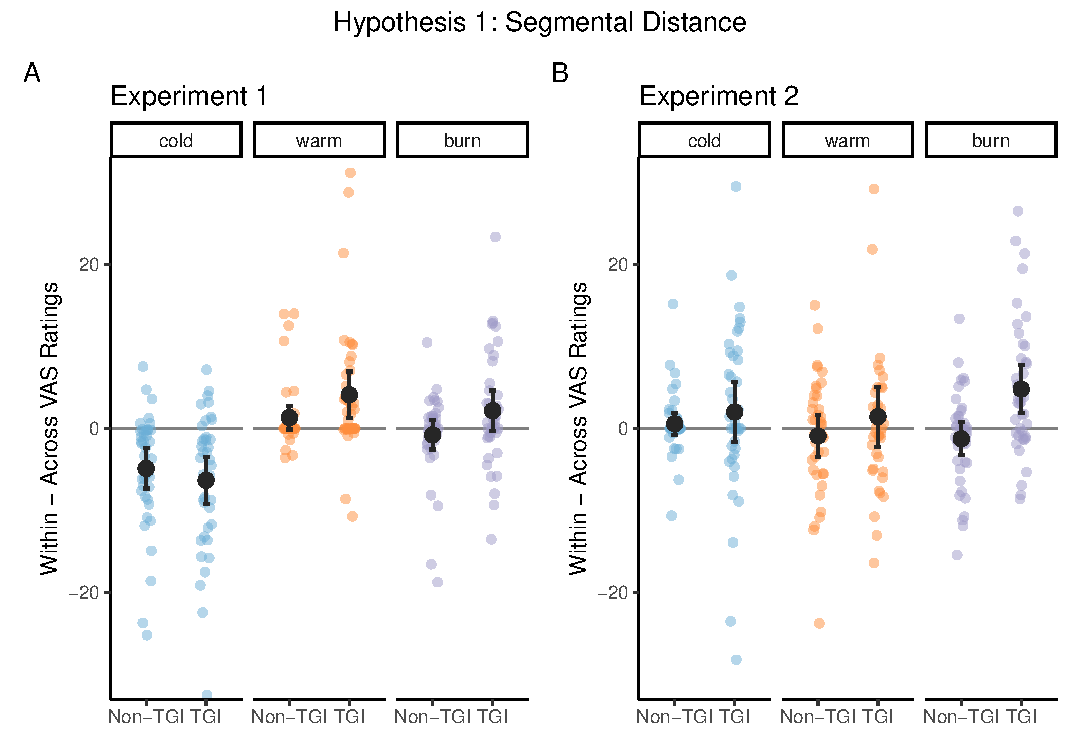
\includegraphics{Manuscript_files/figure-latex/unnamed-chunk-2-1.pdf}
\caption{Four experimental conditions depicting an exemplar cold and
warm thermode placement within and across dermatomes. Within dermatomes,
the relative location of the cold thermode was proximal or distal.
Across dermatomes, the relative location of the corresponding spinal
segments was rostral or caudal.}
\end{figure}

\begin{figure}
\centering
\includegraphics{Manuscript_files/figure-latex/unnamed-chunk-3-1.pdf}
\caption{Difference in VAS ratings between within and across dermatome
conditions for each type of stimulation (Non-TGI and TGI) in each VAS
rating quality (cold, warm and burning). Positive values represent
higher ratings within dermatomes, negative values represent higher
ratings across dermatomes. Small dots are individual subject means,
large dots are population means for each condition and error bars are
95\% confidence intervals. A) first experiment with the cold thermode as
the reference, and B second experiment with the warm thermode as
referece.}
\end{figure}

In keeping with the unique heat and burning features of TGI, our results
exhibited a more robust TGI when stimuli were confined within dermatomes
compared to when applied across dermatomes, corresponding to
non-adjacent spinal segments (Fig. 2).

When rating the cold thermode (Exp. 1), participants reported a
significantly reduced subjective experience of cold for TGI, but not
non-TGI, stimuli applied within a dermatome compared to across
dermatomes (stimulation by dermatome interaction: \(\beta\) = -0.15, p
\textless{} .01). This interaction was not present for for warm
(\(\beta\) = -0.03, p = 0.77), but we did find a strong main effect of
dermatome (\(\beta\) = 0.26, p \textless{} .001) For the burning ratings
we found No significant interaction (\(\beta\) = 0.10, p = 0.15) nor
main effect (\(\beta\) = -0.04, p = 0.39).

In contrast, when rating the warm thermode, participants reported
markedly enhanced burning sensations for TGI, but not non-TGI,
(stimulation by dermatome interaction: \(\beta\) = 0.21, p \textless{}
.001).However, we did not observe suvh a modulation of cold percepts
(\(\beta\) = 0.08, p = 0.28), with no main effect (\(\beta\) = 0.01, p =
0.83) for the warm thermosensory ratings we found no interaction
(\(\beta\) = 0.07, p = 0.16), and no main effect of dermatome (\(\beta\)
= -0.04, p = 0.28).

The findings suggest that the thermosensory quality of the reference
thermode (cold or warm) showed differential sensitivity to thermosensory
and painful aspects of the TGI experience, and collectively suggested
that both the thermosensory enhancement and illusory pain components of
the illusion are modulated at the spinal cord level. This interpretation
is consistent with a previous study using a similar dermatome
manipulation, but a distinct method to quantify TGI perception
(\protect\hyperlink{ref-fardo_organization_2018}{Fardo, Finnerup, and
Haggard 2018}), as well as another study showing modulation of heat and
pain ratings of TGI stimuli by conditioned pain modulation
(\protect\hyperlink{ref-harper_conditioned_2017}{Harper and Hollins
2017}). All together these results support the role of spinal processes
in the generation of distinct perceptual aspects of the TGI.

\hypertarget{undetected-proximodistal-bias-in-tgi}{%
\subsection{Undetected proximodistal bias in
TGI}\label{undetected-proximodistal-bias-in-tgi}}

Previous research demonstrated a phenomenon known as distal inhibition,
wherein heat pain ratings tend to increase when a participant evaluates
a more distal compared to a more proximal stimulus among two warm
stimuli presented on the forearm
(\protect\hyperlink{ref-quevedo_psychophysicshyperalgesia_2004}{A.
Quevedo and Coghill 2004};
\protect\hyperlink{ref-quevedo_illusion_2007}{A. S. Quevedo and Coghill
2007}). In our study, we sought to investigate whether this effect of
distal inhibition would also influence TGI perception within a single
dermatome (Fig. 3). We tested this effect with a two way interaction
between condition (control / TGI) and the location of the cold thermode
when it was placed within dermatome (distal / proximal). In the first
experiment with the cold thermode as the reference we found no
statistical significant interaction effect for the cold ratings
(\(\beta\) = -0.08, p = 0.3, however with a strong main effect of
dermatome (\(\beta\) = -0.18, p \textless{} .001) For the warm ratings
we found no interaction (\(\beta\) = 0.19, p = 0.14), nor main effect of
dermatome (\(\beta\) = -0.08, p = 0.44) For the burning ratings We found
no significant interaction (\(\beta\) = -0.09, p = 0.37), but a
significant main effect ( \(\beta\) = -0.17, p \textless{} .05 )

For the second experiment with the warm thermode as the reference we
found no interaction no interaction (\(\beta\) = -0.06, p = 0.49), nor
main effect (\(\beta\) = 0.00, p = 0.96) for the burning ratings. For
the warm ratings we found no interaction (\(\beta\) = 0.00, p = 0.96), ,
nor main effect of dermatome (\(\beta\) = -0.04, p = 0.42) and for the
cold ratings no interaction (\(\beta\) = 0.10, p = 0.34) but a main
effect (\(\beta\) = -0.18, p \textless{} .05 ).

\begin{figure}
\centering
\includegraphics{Manuscript_files/figure-latex/unnamed-chunk-4-1.pdf}
\caption{Difference in VAS ratings between the proximal and distal
dermatome conditions and the stimulation type (Non-TGI, TGI) for all VAS
rating types (Cold, warm, Burning). A, first experiment with the cold
thermode as the reference, and B with the warm thermode as referce.
Small points show data from each participant, large dots are means
across trials for each condition, and error bars show 95\% confidence
intervals.}
\end{figure}

\hypertarget{directional-effects-in-inter-segmental-sensory-integration}{%
\subsection{Directional effects in inter-segmental sensory
integration}\label{directional-effects-in-inter-segmental-sensory-integration}}

A main objective of this study was assessing spatial order effects along
the rostrocaudal axis at the spinal level. We delivered an equal number
of trials in which the cold stimulus was applied on a dermatome that
mapped more rostrally or caudally compared to the warm or neutral
stimuli. Like the previous analysis we investigated this relationship
with a two way interaction here with the rostral - caudal axis being
investigated.

Results showed no statistical significant interaction effect for the
cold ratings in the first experiment with the reference thermode being
cold (\(\beta\) = -0.10, p = 0.19, but a main effect (\(\beta\) = -0.15,
p \textless{} .01). For the warm ratings we found no statistically
significant effect for warm watings (\(\beta\) = 0.06, p = 0.65), but a
statistical significant main effect (\(\beta\) = 0.21, p \textless{} .05
) The burning ratings showed no significant interaction (\(\beta\) =
0.06, p = 0.54), nor main effect (\(\beta\) = -0.12, p = 0.11).

In Experiment 2, with the warm thermode as the reference we found no
significant interaction effect for the burning ratings (\(\beta\) =
-0.14, p = 0.1), but a significant main effect (\(\beta\) = 0.17, p
\textless{} .01) For the warm ratings we found no statistically
significant interaction (\(\beta\) = 0.01, p = 0.94), but a strong main
effect (\(\beta\) = 0.19, p \textless{} .001) For the cold ratings we
found a significant interaction (\(\beta\) = -0.23, p \textless{} .05 )

\begin{figure}
\centering
\includegraphics{Manuscript_files/figure-latex/unnamed-chunk-5-1.pdf}
\caption{Difference in VAS ratings between the Caudal and Rostral
dermatome conditions and the stimulation type (Non-TGI, TGI) for all VAS
rating types (Cold, warm, Burning). A, first experiment with the cold
thermode as the reference, and B with the warm thermode as referce.
Small points show data from each participant, large dots are means
across trials for each condition, and error bars show 95\% confidence
intervals.}
\end{figure}

The results indicated a notably enhanced TGI effect when the cold
stimulus induced more caudal activity within the spinal cord, as
depicted in Figure 3. These findings were consistent across both
experiments for thermosensory ratings, albeit with minor deviations that
corresponded with the particular stimulation quality being assessed. The
observed enhancement of warmth perception in Experiment 2 could be
ascribed to the participants' assessment of the warmer thermode as
opposed to the colder one of Experiment 1. For burning ratings,
significant results were seen in Experiment 2, but not in Experiment 1.
One possible reason for this discrepancy could be the relatively low
power in Experiment 1, as the power analysis was specifically focused on
thermosensory ratings. Alternatively, assessing the warmer thermode
might be a more accurate method for measuring TGI perception.

\hypertarget{spinal-organisation-and-tgi-perception}{%
\subsection{Spinal organisation and TGI
perception}\label{spinal-organisation-and-tgi-perception}}

The complexities of spinal neuroanatomy provide insightful perspectives
concerning the two main findings of these experiments: (1) enhanced heat
and burning sensations when cold-warm thermosensory integration takes
place more focally within the spinal cord, and (2) discernible
directional inter-segmental effects when distinct cold and warm stimuli
elicited broader activity along the spinal cord. Small primary
afferents, responsible for mediating temperature and pain sensations,
split into ascending and descending branches that cover one to two
segments before they enter the dorsal horn
(\protect\hyperlink{ref-kerr_neuroanatomical_1975}{Kerr 1975};
\protect\hyperlink{ref-lamotte_distribution_1977}{Lamotte 1977}). This
pattern forms the Lissauer's tract, a structure hypothesised to regulate
sensory transmission to the dorsal horn and influence spinal receptive
field size (\protect\hyperlink{ref-wall_brief_1999}{Wall, Lidierth, and
Hillman 1999}).

Additionally, the endings of small primary afferents within the
superficial laminae of the dorsal horn form synapses with both
propriospinal neurons and projection neurons that target supraspinal
structures known to significantly influence TGI perception
(\protect\hyperlink{ref-craig_functional_1996}{Craig et al. 1996};
\protect\hyperlink{ref-lindstedt_evidence_2011}{Lindstedt et al. 2011};
\protect\hyperlink{ref-leung_supraspinal_2014}{Leung et al. 2014} + any
other neuroimaging studies of the TGI).

Evidence from animal studies shows that propriospinal neurons, confined
within the spinal cord, exhibit bidirectional collateral branches along
the rostrocaudal plane
(\protect\hyperlink{ref-saywell_electrophysiological_2011}{Saywell et
al. 2011}; \protect\hyperlink{ref-skinner_ascending_1989}{Skinner et al.
1989}). These connections shape the network of interneurons that
modulates sensory information delivered to the dorsal horn
(\protect\hyperlink{ref-todd_neuronal_2010}{Todd 2010};
\protect\hyperlink{ref-peirs_neural_2016}{Peirs and Seal 2016}).

Our finding of enhanced TGI perception with cold-warm stimuli applied
within dermatomes might reflect the combined effects of the Lissauer's
tract's short rostrocaudal span (comprising one to two segments,
consistent with a single dermatome's boundary) and the characteristics
of spinal circuits. These circuits, created by propriospinal neurons,
may promote sensory integration within a spinal receptive field while
simultaneously inhibiting activity in adjacent fields. This mechanism
aligns with the concept of lateral inhibition, a ubiquitous process in
sensory processing seen across both the peripheral and central nervous
systems, and multiple sensory modalities, including thermoception and
nociception (\protect\hyperlink{ref-bekesy_lateral_1962}{Békésy 1962};
\protect\hyperlink{ref-quevedo_lateral_2017}{A. S. Quevedo et al. 2017};
\protect\hyperlink{ref-adamczyk_not_2021}{Adamczyk et al. 2021}).
Further, our observation that spatial factors, such as the more caudal
localisation of cold activity relative to warm activity in the spinal
cord, influences TGI perception, suggests possible neuroanatomical and
functional asymmetries. This could mean a greater number of ascending
fibres than descending fibres carrying thermosensory information in the
Lissauer's tract, an uneven distribution of ascending and descending
collaterals of propriospinal neurons (Anatomical Hypotheses), or varying
effects of inter-segmental inhibition along the rostrocaudal axis
(Functional Hypothesis). Additional research is needed to illuminate the
specific anatomical and functional features of the spinal cord that
resulted in the observed effects of this study.

\hypertarget{conclusion}{%
\section{Conclusion}\label{conclusion}}

Illusions in the thermo-nociceptive system can be leveraged to improve
our understanding of mechanisms contributing to pain perception. Here,
we presented results supporting the notion that the spinal cord plays a
crucial role in the integration and processing of thermal information,
contributing to the perception of both thermosensory enhancement and the
illusory pain within the TGI. Additionally, we reported findings on
directional inter-segmental effects in spinal integration underlying
TGI. Further research is needed to elucidate the neuroanatomical and
functional properties of the spinal cord, as well as the intricate
interplay between supraspinal and spinal processes, that give rise to
TGI perception.

\newpage

\hypertarget{methods}{%
\section{Methods}\label{methods}}

\hypertarget{participants}{%
\subsection{Participants}\label{participants}}

The study entailed two separate experiments, collectively involving 80
healthy volunteers. The sample consisted of 27 females and 13 males,
mean age = 25.38 years old (SD = 4.67, range = 18 - 36) in Experiment 1,
and 25 females and 14 males and 1 non-binary (Female at birth), mean age
= 25.73 years old (SD = 4.12, range = 21 - 39), in Experiment 2. The
research methodology complied with the principles set forth in the
Declaration of Helsinki and received ethical approval from the
Institutional Review Board (IRB) at the Danish Neuroscience Center,
Aarhus University, Denmark. Prior to commencing the study, all
participants were fully informed about the procedures and provided their
voluntary consent.

\hypertarget{stimuli-and-procedure}{%
\subsection{Stimuli and procedure}\label{stimuli-and-procedure}}

All thermal stimuli were delivered using two NTE-3 Thermal Sensitivity
Testers (PhysiTemp Instruments LLC) controlled by PhysiTemp NTE-3
software (version 5.4b). The procedure involved measurements of heat and
cold pain thresholds, calibration of cold-warm temperature pairs
eliciting TGI, and an experimental task where TGI and non-TGI stimuli
were applied on dermatomes that mapped onto adjacent or non-adjacent
spinal segments. To measure cold and heat pain thresholds, we gradually
adjusted the temperature of one thermode until the participant indicated
an experience of pain by pressing a stop button or reached the maximum
temperature cut-offs of 5ºC or 50ºC. We calibrated TGI stimuli by
identifying a cold-warm temperature pair based on specific criteria: (1)
consistently eliciting a burning sensation of at least 15 on a scale
ranging from 0 to 100, (2) consistently avoiding a burning sensation
(less than 15) when the cold-neutral (Exp. 1) or warm-neutral (Exp. 2)
stimuli were presented, (3) both cold and warm temperatures falling
within the innocuous range based on individual cold and heat pain
thresholds. For pain threshold measurements and TGI calibration, we
positioned the probes within a single dermatome. To address our
experimental questions, we presented the calibrated TGI stimuli, as well
as cold-neutral (Exp. 1) or warm-neutral (Exp. 2) non-TGI stimuli using
two thermodes. In non-TGI stimuli the cold or warm temperatures were set
to match the temperature used for TGI stimulation, but paired with a
neutral temperature set at 30ºC. The two thermodes were positioned on
the internal surface of either forearm, with a constant spacing value
between 4 and 5 cm in each direction, depending on the participant's
forearm size. The positioning of the thermodes was either within the
same dermatome (i.e., C6 and T1) or across dermatomes mapped onto
non-adjacent spinal segments (i.e.~C6 - T1). Further, we manipulated the
spatial arrangement of the temperature pairs, by systematically
presenting an equal number of trials where the cold thermode was applied
on a proximal or distal location within a dermatome, or was applied on a
dermatome that mapped onto a rostral or caudal segment along the spinal
cord. We based the demarcation of the dermatome boundaries on the
American Spinal Injury Association (ASIA) map (Fardo et al., 2018) and
positioned the thermodes in relation to standard anatomical landmarks.
Proximo-distal coordinates referred to locations on the skin closer to
the elbow or the wrist, whereas rostral-caudal coordinates referred to
spinal segments closer to the head or the lower back. The possible
spatial arrangements corresponded to the four conditions depicted in
Figure 1. The order of the stimuli (TGI vs.~non-TGI), the dermatome
condition (within vs.~across) and the relative placement of the colder
temperature (proximal vs.~distal or rostral vs.~caudal) were
pseudo-randomised and counterbalanced between participants. During each
trial, the experimenter positioned two thermodes, mounted on a stand
using two independent clamps, on the participant's skin for 10 seconds.
An auditory cue (300Hz, 100ms) indicated the end of the stimulation
period, after which the experimenter removed the thermodes from the
participant's skin. Participants then rated the most intense cold, warm
or burning sensation they perceived during the stimulation period using
three separated computerised VAS scales. VAS scales were presented one
at a time on a computer screen and appeared as a horizontal line,
anchored at 0, representing no sensation (e.g., no burning), and 100,
signifying an extreme sensation (e.g., extreme burning). The order of
the three VAS scales was randomised across trials. For each scale,
participants provided their responses using the arrow keys on a keyboard
and rated the intensity of their sensations from a specific location
(labeled `A' or `B'), based on the experimenter's instruction. Unbeknown
to the participant, this location systematically corresponded to either
the colder temperature (Exp. 1) or the warmer temperature (Exp. 2).
Participants had max 8 seconds to provide each rating, and if they did
not complete a rating within the allowed timeframe, the trial was
repeated. Following the completion of the last of the three VAS ratings,
we presented a 200 ms fixation dot. Each thermode configuration was
tested three consecutive times, on three different skin locations. An
auditory tone of 500Hz lasting 100ms was played to indicate to the
experimenter when to rearrange the thermode configuration to stimulate
different dermatomes depending on a pseudo-randomisation order. Each of
the four experimental conditions was repeated 12 times, with both the
right and left forearms stimulated, and a minimum of five trials between
the re-stimulation of the same skin location. This ensured that the same
skin locations were not stimulated consecutively to minimise carry-over
effects. Experiments 1 and 2 were conducted in two independent groups of
participants and followed exactly the same procedure except for two
elements. In Experiment 1, participants rated the sensations localised
underneath the colder thermode, and the non-TGI stimuli corresponded to
cold-neutral pairs. In Experiment 2, participants rated the sensations
localised underneath the warmer thermode, and the non-TGI stimuli
corresponded to warm-neutral pairs.

\hypertarget{sample-size}{%
\subsection{Sample size}\label{sample-size}}

An initial pilot study informed the pre-registered calculation of the
sample size. To test the directional TGI hypothesis with 95\% power and
detect an effect size of .12 or greater, we determined that we needed a
minimum number of 32 TGI-responsive participants. We defined
TGI-responders as those individuals for whom the median burning ratings
for TGI stimuli significantly exceeded 0. Non-responders were
individuals that did not meet this criterion when tested with the max
cold-warm temperatures allowed in the experiment. The predefined cut-off
for TGI stimulation was (xx-xx). In Experiment 1, recruitment continued
until we achieved the target of 32 TGI-responsive participants. We
verified this criterion every 10 participants, resulting in a total
sample size of 40 participants. In Experiment 2, we stopped recruitment
once we collected data from 40 participants. This decision was based on
meeting both required criteria: (1) matching the sample size of Exp. 1
for consistency, and (2) achieving the minimum requirement of 32
TGI-responsive participants as determined by the power analysis.

\hypertarget{data-analyses}{%
\subsection{Data analyses}\label{data-analyses}}

We re-scaled data from cold, warm and burning VAS ratings from their
original values to a range of 0 to 1. Following re-scaling, we applied
zero-inflated mixed-effects beta regression models separately for each
set of VAS ratings. In these models, we incorporated three fixed
effects. These included the type of stimulation (non-TGI vs.~TGI), the
dermatome condition (within the same dermatome vs.~across different
dermatomes) and the spatial positioning of the cold or neutral thermode
(proximal vs.~distal within dermatomes; rostral vs.~caudal across
dermatomes). These choices allowed us to assess the individual and
interactive effects of these three factors on VAS ratings. Further, we
added random intercepts to our models to account for between-subject
variability and the effects of repeated measures. The variables
introduced as random intercepts included the participant ID, the
counterbalancing order and the trial number. The choices of the
zero-inflated approach and the use of beta regressions were necessitated
by the specific distribution of VAS ratings. The beta distribution is
suitable for modelling VAS rating data, as they are proportional in
nature. Additionally, the zero-inflation was needed due to the presence
of an excess number of zero values in specific ratings and conditions.
Specifically, we anticipated an overrepresentation of zero values for
thermosensory ratings that were counterfactual to the objective
stimulation quality (i.e., cold ratings of warm stimuli and warm ratings
of cold stimuli) and burning ratings of non-TGI stimuli. The latter
stimuli were designed to not elicit an illusion or trigger a weaker
illusion as compared to the TGI stimuli. We carried out the statistical
analyses using the `glmmTMB' package in R (version 1.1.7), and
statistical significance was set at p \textless{} .05. The experimental
procedure, power analyses to determine sample size and statistical
approach were preregistered for both
\href{https://osf.io/4xcn5/}{Experiment 1} and
\href{https://osf.io/dhg8u/}{Experiment 2}. All data and code for the
analysis are available in the
\href{https://github.com/Body-Pain-Perception-Lab/tgi-spinal/tree/Markdown-manuscript}{github
repository}, ensuring the reproducibility of our findings.

\newpage

\hypertarget{authors-contributions}{%
\section{Authors contributions}\label{authors-contributions}}

Author contributions listed alphabetically according to
\href{https://credit.niso.org}{CRediT taxonomy}:

\begin{itemize}
\tightlist
\item
  Conceptualization: DEC, JFE, FF, PH, AGM.
\item
  Data curation: JEF, AGM.
\item
  Formal analysis: JFE, FF, AGM.
\item
  Funding acquisition: FF.
\item
  Investigation: DEC, JFE, AGM.
\item
  Methodology: DEC, JFE, FF, AGM, AVS.
\item
  Project administration: FF, AGM.
\item
  Resources: FF, AGM.
\item
  Software: JFE, FF, AGM.
\item
  Supervision: FF, AGM.
\item
  Visualization: FF, AGM.
\item
  Writing -- original draft: FF, AGM.
\item
  Writing -- review \& editing: FF, AGM. (+ others who will provide
  feedback)
\end{itemize}

\hypertarget{acknowledgements}{%
\section{Acknowledgements}\label{acknowledgements}}

We would like to thank XXX for their help with participant recruitment
and data collection. This study was supported by a European Research
Council Starting Grant (ERC-2020-StG-948788).

\newpage

\hypertarget{references}{%
\section{References}\label{references}}

\hypertarget{refs}{}
\begin{CSLReferences}{1}{0}
\leavevmode\vadjust pre{\hypertarget{ref-adam_relationships_2014}{}}%
Adam, Frédéric, Pascal Alfonsi, Delphine Kern, and Didier Bouhassira.
2014. {``Relationships Between the Paradoxical Painful and Nonpainful
Sensations Induced by a Thermal Grill.''} \emph{PAIN} 155 (12): 2612.
\url{https://doi.org/10.1016/j.pain.2014.09.026}.

\leavevmode\vadjust pre{\hypertarget{ref-adamczyk_not_2021}{}}%
Adamczyk, Wacław M., Tibor M. Szikszay, Tiffany Kung, Gabriela F.
Carvalho, and Kerstin Luedtke. 2021. {``Not as "Blurred" as Expected?
{Acuity} and Spatial Summation in the Pain System.''} \emph{PAIN} 162
(3): 794--802. \url{https://doi.org/10.1097/j.pain.0000000000002069}.

\leavevmode\vadjust pre{\hypertarget{ref-bach_thermal_2011}{}}%
Bach, Patrick, Susanne Becker, Dieter Kleinböhl, and Rupert Hölzl. 2011.
{``The Thermal Grill Illusion and What Is Painful about It.''}
\emph{Neuroscience Letters} 505 (1): 31--35.
\url{https://doi.org/10.1016/j.neulet.2011.09.061}.

\leavevmode\vadjust pre{\hypertarget{ref-bekesy_lateral_1962}{}}%
Békésy, G. V. 1962. {``Lateral Inhibition of Heat Sensations on the
Skin.''} \emph{Journal of Applied Physiology} 17 (6): 1003--8.
\url{https://doi.org/10.1152/jappl.1962.17.6.1003}.

\leavevmode\vadjust pre{\hypertarget{ref-bouhassira_investigation_2005}{}}%
Bouhassira, Didier, Delphine Kern, Jean Rouaud, Emilie Pelle-Lancien,
and Françoise Morain. 2005. {``Investigation of the Paradoxical Painful
Sensation ({`Illusion of Pain'}) Produced by a Thermal Grill.''}
\emph{PAIN} 114 (1): 160.
\url{https://doi.org/10.1016/j.pain.2004.12.014}.

\leavevmode\vadjust pre{\hypertarget{ref-craig_new_1998}{}}%
Craig, A. D. 1998. {``A New Version of the Thalamic Disinhibition
Hypothesis of Central Pain.''} \emph{Pain Forum} 7 (1): 1--14.
\url{https://doi.org/10.1016/S1082-3174(98)70004-2}.

\leavevmode\vadjust pre{\hypertarget{ref-craig_thermal_1994}{}}%
Craig, A. D., and M. C. Bushnell. 1994. {``The Thermal Grill Illusion:
Unmasking the Burn of Cold Pain.''} \emph{Science} 265 (5169): 252--55.
\url{https://doi.org/10.1126/science.8023144}.

\leavevmode\vadjust pre{\hypertarget{ref-craig_functional_1996}{}}%
Craig, A. D., E. M. Reiman, A. Evans, and M. C. Bushnell. 1996.
{``Functional Imaging of an Illusion of Pain.''} \emph{Nature} 384
(6606): 258--60. \url{https://doi.org/10.1038/384258a0}.

\leavevmode\vadjust pre{\hypertarget{ref-defrin_spatial_2008}{}}%
Defrin, Ruth, Anat Benstein-Sheraizin, Adva Bezalel, Ofira Mantzur, and
Lars Arendt-Nielsen. 2008. {``The Spatial Characteristics of the Painful
Thermal Grill Illusion.''} \emph{PAIN} 138 (3): 577.
\url{https://doi.org/10.1016/j.pain.2008.02.012}.

\leavevmode\vadjust pre{\hypertarget{ref-fardo_beyond_2020}{}}%
Fardo, Francesca, Brianna Beck, Micah Allen, and Nanna Brix Finnerup.
2020. {``Beyond Labeled Lines: {A} Population Coding Account of the
Thermal Grill Illusion.''} \emph{Neuroscience and Biobehavioral Reviews}
108 (January): 472--79.
\url{https://doi.org/10.1016/j.neubiorev.2019.11.017}.

\leavevmode\vadjust pre{\hypertarget{ref-fardo_organization_2018}{}}%
Fardo, Francesca, Nanna Brix Finnerup, and Patrick Haggard. 2018.
{``Organization of the Thermal Grill Illusion by Spinal Segments.''}
\emph{Annals of Neurology} 84 (3): 463--72.
\url{https://doi.org/10.1002/ana.25307}.

\leavevmode\vadjust pre{\hypertarget{ref-ferre_ineffectiveness_2018}{}}%
Ferrè, E. R., G. D. Iannetti, J. A. van Dijk, and P. Haggard. 2018.
{``Ineffectiveness of Tactile Gating Shows Cortical Basis of Nociceptive
Signaling in the {Thermal} {Grill} {Illusion}.''} \emph{Scientific
Reports} 8 (April): 6584.
\url{https://doi.org/10.1038/s41598-018-24635-1}.

\leavevmode\vadjust pre{\hypertarget{ref-fruhstorfer_significance_2003}{}}%
Fruhstorfer, Heinrich, Eva-Liz Harju, and Ulf F. Lindblom. 2003. {``The
Significance of {A}-Delta and {C} Fibres for the Perception of Synthetic
Heat.''} \emph{European Journal of Pain} 7 (1): 63--71.
\url{https://doi.org/10.1016/s1090-3801(02)00056-3}.

\leavevmode\vadjust pre{\hypertarget{ref-green_localization_1977}{}}%
Green, Barry G. 1977. {``Localization of Thermal Sensation: {An}
Illusion and Synthetic Heat.''} \emph{Perception \& Psychophysics} 22
(4): 331--37. \url{https://doi.org/10.3758/BF03199698}.

\leavevmode\vadjust pre{\hypertarget{ref-green_synthetic_2002}{}}%
---------. 2002. {``Synthetic Heat at Mild Temperatures.''}
\emph{Somatosensory \& Motor Research} 19 (2): 130--38.
\url{https://doi.org/10.1080/08990220220220131524}.

\leavevmode\vadjust pre{\hypertarget{ref-green_temperature_2004}{}}%
---------. 2004. {``Temperature Perception and Nociception.''}
\emph{Journal of Neurobiology} 61 (1): 13--29.
\url{https://doi.org/10.1002/neu.20081}.

\leavevmode\vadjust pre{\hypertarget{ref-harper_conditioned_2017}{}}%
Harper, D. E., and M. Hollins. 2017. {``Conditioned Pain Modulation
Dampens the Thermal Grill Illusion.''} \emph{European Journal of Pain}
21 (9): 1591--601. \url{https://doi.org/10.1002/ejp.1060}.

\leavevmode\vadjust pre{\hypertarget{ref-kern_pharmacological_2008}{}}%
Kern, Delphine, Emilie Pelle-lancien, Virginie Luce, and Didier
Bouhassira. 2008. {``Pharmacological Dissection of the Paradoxical Pain
Induced by a Thermal Grill.''} \emph{PAIN} 135 (3): 291.
\url{https://doi.org/10.1016/j.pain.2007.12.001}.

\leavevmode\vadjust pre{\hypertarget{ref-kern_effects_2008}{}}%
Kern, Delphine, Frédéric Plantevin, and Didier Bouhassira. 2008.
{``Effects of Morphine on the Experimental Illusion of Pain Produced by
a Thermal Grill.''} \emph{PAIN} 139 (3): 653.
\url{https://doi.org/10.1016/j.pain.2008.07.001}.

\leavevmode\vadjust pre{\hypertarget{ref-kerr_neuroanatomical_1975}{}}%
Kerr, Frederick W. L. 1975. {``Neuroanatomical Substrates of Nociception
in the Spinal Cord.''} \emph{PAIN} 1 (4): 325.
\url{https://doi.org/10.1016/0304-3959(75)90072-X}.

\leavevmode\vadjust pre{\hypertarget{ref-lamotte_distribution_1977}{}}%
Lamotte, Carole. 1977. {``Distribution of the Tract of Lissauer and the
Dorsal Root Fibers in the Primate Spinal Cord.''} \emph{Journal of
Comparative Neurology} 172 (3): 529--61.
\url{https://doi.org/10.1002/cne.901720308}.

\leavevmode\vadjust pre{\hypertarget{ref-leung_supraspinal_2014}{}}%
Leung, Albert, Shivshil Shukla, Eric Li, Jeng-Ren Duann, and Tony Yaksh.
2014. {``Supraspinal {Characterization} of the {Thermal} {Grill}
{Illusion} with {fMRI}.''} \emph{Molecular Pain} 10 (January):
1744-8069-10-18. \url{https://doi.org/10.1186/1744-8069-10-18}.

\leavevmode\vadjust pre{\hypertarget{ref-lindstedt_evidence_2011}{}}%
Lindstedt, Fredrik, Bo Johansson, Sofia Martinsen, Eva Kosek, Peter
Fransson, and Martin Ingvar. 2011. {``Evidence for Thalamic Involvement
in the Thermal Grill Illusion: An {FMRI} Study.''} \emph{PloS One} 6
(11): e27075. \url{https://doi.org/10.1371/journal.pone.0027075}.

\leavevmode\vadjust pre{\hypertarget{ref-marotta_transforming_2015}{}}%
Marotta, Angela, Elisa Raffaella Ferrè, and Patrick Haggard. 2015.
{``Transforming the {Thermal} {Grill} {Effect} by {Crossing} the
{Fingers}.''} \emph{Current Biology} 25 (8): 1069--73.
\url{https://doi.org/10.1016/j.cub.2015.02.055}.

\leavevmode\vadjust pre{\hypertarget{ref-peirs_neural_2016}{}}%
Peirs, Cedric, and Rebecca P. Seal. 2016. {``Neural Circuits for Pain:
{Recent} Advances and Current Views.''} \emph{Science} 354 (6312):
578--84. \url{https://doi.org/10.1126/science.aaf8933}.

\leavevmode\vadjust pre{\hypertarget{ref-quevedo_psychophysicshyperalgesia_2004}{}}%
Quevedo, A., and R. Coghill. 2004. {``Psychophysics/Hyperalgesia:
{Spatial} Interactions Between Multiple Painful Stimuli.''} \emph{The
Journal of Pain} 5 (3): S32.
\url{https://doi.org/10.1016/j.jpain.2004.02.094}.

\leavevmode\vadjust pre{\hypertarget{ref-quevedo_illusion_2007}{}}%
Quevedo, Alexandre S., and Robert C. Coghill. 2007. {``An {Illusion} of
{Proximal} {Radiation} of {Pain} {Due} to {Distally} {Directed}
{Inhibition}.''} \emph{The Journal of Pain} 8 (3): 280--86.
\url{https://doi.org/10.1016/j.jpain.2006.09.003}.

\leavevmode\vadjust pre{\hypertarget{ref-quevedo_lateral_2017}{}}%
Quevedo, Alexandre S., Carsten Dahl Mørch, Ole K. Andersen, and Robert
C. Coghill. 2017. {``Lateral Inhibition During Nociceptive
Processing.''} \emph{PAIN} 158 (6): 1046.
\url{https://doi.org/10.1097/j.pain.0000000000000876}.

\leavevmode\vadjust pre{\hypertarget{ref-saywell_electrophysiological_2011}{}}%
Saywell, S. A., T. W. Ford, C. F. Meehan, A. J. Todd, and P. A.
Kirkwood. 2011. {``Electrophysiological and {Morphological}
{Characterization} of {Propriospinal} {Interneurons} in the {Thoracic}
{Spinal} {Cord}.''} \emph{Journal of Neurophysiology} 105 (2): 806--26.
\url{https://doi.org/10.1152/jn.00738.2010}.

\leavevmode\vadjust pre{\hypertarget{ref-skinner_ascending_1989}{}}%
Skinner, R. D., R. Nelson, M. Griebel, and E. Garcia-Rill. 1989.
{``Ascending Projections of Long Descending Propriospinal Tract ({LDPT})
Neurons.''} \emph{Brain Research Bulletin} 22 (2): 253--58.
\url{https://doi.org/10.1016/0361-9230(89)90050-6}.

\leavevmode\vadjust pre{\hypertarget{ref-todd_neuronal_2010}{}}%
Todd, Andrew J. 2010. {``Neuronal Circuitry for Pain Processing in the
Dorsal Horn.''} \emph{Nature Reviews Neuroscience} 11 (12): 823--36.
\url{https://doi.org/10.1038/nrn2947}.

\leavevmode\vadjust pre{\hypertarget{ref-wall_brief_1999}{}}%
Wall, Patrick D., Malcolm Lidierth, and Peter Hillman. 1999. {``Brief
and Prolonged Effects of {Lissauer} Tract Stimulation on Dorsal Horn
Cells.''} \emph{PAIN} 83 (3): 579--89.
\url{https://doi.org/10.1016/S0304-3959(99)00170-0}.

\end{CSLReferences}

\newpage

\hypertarget{supplementary-material}{%
\section{Supplementary material}\label{supplementary-material}}

\global\setlength{\Oldarrayrulewidth}{\arrayrulewidth}

\global\setlength{\Oldtabcolsep}{\tabcolsep}

\setlength{\tabcolsep}{0pt}

\renewcommand*{\arraystretch}{1.5}



\providecommand{\ascline}[3]{\noalign{\global\arrayrulewidth #1}\arrayrulecolor[HTML]{#2}\cline{#3}}

\begin{longtable}[c]{|p{2.50in}|p{1.10in}|p{1.10in}|p{1.10in}|p{1.10in}}



\ascline{1.5pt}{666666}{1-5}

\multicolumn{5}{>{\centering}m{\dimexpr 6.9in+8\tabcolsep}}{\textcolor[HTML]{000000}{\fontsize{10}{10}\selectfont{\global\setmainfont{Times New Roman}{Cold\ reference\ on\ cold\ ratings}}}} \\

\ascline{1.5pt}{666666}{1-5}



\multicolumn{5}{>{\centering}m{\dimexpr 6.9in+8\tabcolsep}}{\textcolor[HTML]{000000}{\fontsize{10}{10}\selectfont{\global\setmainfont{Times New Roman}{beta\textasciitilde manipulation\ *\ cold\_probe\ +\ trial\_n\ +\ (1\ |\ ID)\ +\ (1\ |\ order),\ family\ =\ beta(link\ =\ logit)}}}} \\

\ascline{1.5pt}{666666}{1-5}



\multicolumn{1}{>{\raggedright}m{\dimexpr 2.5in+0\tabcolsep}}{\textcolor[HTML]{000000}{\fontsize{10}{10}\selectfont{\global\setmainfont{Times New Roman}{\ \ }}}} & \multicolumn{1}{>{\raggedright}m{\dimexpr 1.1in+0\tabcolsep}}{\textcolor[HTML]{000000}{\fontsize{10}{10}\selectfont{\global\setmainfont{Times New Roman}{β}}}} & \multicolumn{1}{>{\raggedright}m{\dimexpr 1.1in+0\tabcolsep}}{\textcolor[HTML]{000000}{\fontsize{10}{10}\selectfont{\global\setmainfont{Times New Roman}{SE}}}} & \multicolumn{1}{>{\raggedright}m{\dimexpr 1.1in+0\tabcolsep}}{\textcolor[HTML]{000000}{\fontsize{10}{10}\selectfont{\global\setmainfont{Times New Roman}{Z}}}} & \multicolumn{1}{>{\raggedright}m{\dimexpr 1.1in+0\tabcolsep}}{\textcolor[HTML]{000000}{\fontsize{10}{10}\selectfont{\global\setmainfont{Times New Roman}{p}}}} \\

\ascline{1.5pt}{666666}{1-5}\endfirsthead 

\ascline{1.5pt}{666666}{1-5}

\multicolumn{5}{>{\centering}m{\dimexpr 6.9in+8\tabcolsep}}{\textcolor[HTML]{000000}{\fontsize{10}{10}\selectfont{\global\setmainfont{Times New Roman}{Cold\ reference\ on\ cold\ ratings}}}} \\

\ascline{1.5pt}{666666}{1-5}



\multicolumn{5}{>{\centering}m{\dimexpr 6.9in+8\tabcolsep}}{\textcolor[HTML]{000000}{\fontsize{10}{10}\selectfont{\global\setmainfont{Times New Roman}{beta\textasciitilde manipulation\ *\ cold\_probe\ +\ trial\_n\ +\ (1\ |\ ID)\ +\ (1\ |\ order),\ family\ =\ beta(link\ =\ logit)}}}} \\

\ascline{1.5pt}{666666}{1-5}



\multicolumn{1}{>{\raggedright}m{\dimexpr 2.5in+0\tabcolsep}}{\textcolor[HTML]{000000}{\fontsize{10}{10}\selectfont{\global\setmainfont{Times New Roman}{\ \ }}}} & \multicolumn{1}{>{\raggedright}m{\dimexpr 1.1in+0\tabcolsep}}{\textcolor[HTML]{000000}{\fontsize{10}{10}\selectfont{\global\setmainfont{Times New Roman}{β}}}} & \multicolumn{1}{>{\raggedright}m{\dimexpr 1.1in+0\tabcolsep}}{\textcolor[HTML]{000000}{\fontsize{10}{10}\selectfont{\global\setmainfont{Times New Roman}{SE}}}} & \multicolumn{1}{>{\raggedright}m{\dimexpr 1.1in+0\tabcolsep}}{\textcolor[HTML]{000000}{\fontsize{10}{10}\selectfont{\global\setmainfont{Times New Roman}{Z}}}} & \multicolumn{1}{>{\raggedright}m{\dimexpr 1.1in+0\tabcolsep}}{\textcolor[HTML]{000000}{\fontsize{10}{10}\selectfont{\global\setmainfont{Times New Roman}{p}}}} \\

\ascline{1.5pt}{666666}{1-5}\endhead



\multicolumn{1}{>{\raggedright}m{\dimexpr 2.5in+0\tabcolsep}}{\textcolor[HTML]{000000}{\fontsize{10}{10}\selectfont{\global\setmainfont{Times New Roman}{Intercept}}}} & \multicolumn{1}{>{\raggedright}m{\dimexpr 1.1in+0\tabcolsep}}{\textcolor[HTML]{000000}{\fontsize{10}{10}\selectfont{\global\setmainfont{Times New Roman}{-0.88}}}} & \multicolumn{1}{>{\raggedright}m{\dimexpr 1.1in+0\tabcolsep}}{\textcolor[HTML]{000000}{\fontsize{10}{10}\selectfont{\global\setmainfont{Times New Roman}{0.17}}}} & \multicolumn{1}{>{\raggedright}m{\dimexpr 1.1in+0\tabcolsep}}{\textcolor[HTML]{000000}{\fontsize{10}{10}\selectfont{\global\setmainfont{Times New Roman}{-5.2}}}} & \multicolumn{1}{>{\raggedright}m{\dimexpr 1.1in+0\tabcolsep}}{\textcolor[HTML]{000000}{\fontsize{10}{10}\selectfont{\global\setmainfont{Times New Roman}{2.5e-07}}}} \\





\multicolumn{1}{>{\raggedright}m{\dimexpr 2.5in+0\tabcolsep}}{\textcolor[HTML]{000000}{\fontsize{10}{10}\selectfont{\global\setmainfont{Times New Roman}{TGI-CNT}}}} & \multicolumn{1}{>{\raggedright}m{\dimexpr 1.1in+0\tabcolsep}}{\textcolor[HTML]{000000}{\fontsize{10}{10}\selectfont{\global\setmainfont{Times New Roman}{-0.19}}}} & \multicolumn{1}{>{\raggedright}m{\dimexpr 1.1in+0\tabcolsep}}{\textcolor[HTML]{000000}{\fontsize{10}{10}\selectfont{\global\setmainfont{Times New Roman}{0.027}}}} & \multicolumn{1}{>{\raggedright}m{\dimexpr 1.1in+0\tabcolsep}}{\textcolor[HTML]{000000}{\fontsize{10}{10}\selectfont{\global\setmainfont{Times New Roman}{\ -7}}}} & \multicolumn{1}{>{\raggedright}m{\dimexpr 1.1in+0\tabcolsep}}{\textcolor[HTML]{000000}{\fontsize{10}{10}\selectfont{\global\setmainfont{Times New Roman}{1.9e-12}}}} \\





\multicolumn{1}{>{\raggedright}m{\dimexpr 2.5in+0\tabcolsep}}{\textcolor[HTML]{000000}{\fontsize{10}{10}\selectfont{\global\setmainfont{Times New Roman}{Within-Across}}}} & \multicolumn{1}{>{\raggedright}m{\dimexpr 1.1in+0\tabcolsep}}{\textcolor[HTML]{000000}{\fontsize{10}{10}\selectfont{\global\setmainfont{Times New Roman}{-0.15}}}} & \multicolumn{1}{>{\raggedright}m{\dimexpr 1.1in+0\tabcolsep}}{\textcolor[HTML]{000000}{\fontsize{10}{10}\selectfont{\global\setmainfont{Times New Roman}{0.037}}}} & \multicolumn{1}{>{\raggedright}m{\dimexpr 1.1in+0\tabcolsep}}{\textcolor[HTML]{000000}{\fontsize{10}{10}\selectfont{\global\setmainfont{Times New Roman}{\ -4}}}} & \multicolumn{1}{>{\raggedright}m{\dimexpr 1.1in+0\tabcolsep}}{\textcolor[HTML]{000000}{\fontsize{10}{10}\selectfont{\global\setmainfont{Times New Roman}{6e-05}}}} \\





\multicolumn{1}{>{\raggedright}m{\dimexpr 2.5in+0\tabcolsep}}{\textcolor[HTML]{000000}{\fontsize{10}{10}\selectfont{\global\setmainfont{Times New Roman}{Caudal-Rostral}}}} & \multicolumn{1}{>{\raggedright}m{\dimexpr 1.1in+0\tabcolsep}}{\textcolor[HTML]{000000}{\fontsize{10}{10}\selectfont{\global\setmainfont{Times New Roman}{-0.15}}}} & \multicolumn{1}{>{\raggedright}m{\dimexpr 1.1in+0\tabcolsep}}{\textcolor[HTML]{000000}{\fontsize{10}{10}\selectfont{\global\setmainfont{Times New Roman}{0.052}}}} & \multicolumn{1}{>{\raggedright}m{\dimexpr 1.1in+0\tabcolsep}}{\textcolor[HTML]{000000}{\fontsize{10}{10}\selectfont{\global\setmainfont{Times New Roman}{-2.9}}}} & \multicolumn{1}{>{\raggedright}m{\dimexpr 1.1in+0\tabcolsep}}{\textcolor[HTML]{000000}{\fontsize{10}{10}\selectfont{\global\setmainfont{Times New Roman}{0.0038}}}} \\





\multicolumn{1}{>{\raggedright}m{\dimexpr 2.5in+0\tabcolsep}}{\textcolor[HTML]{000000}{\fontsize{10}{10}\selectfont{\global\setmainfont{Times New Roman}{Proximal-Distal}}}} & \multicolumn{1}{>{\raggedright}m{\dimexpr 1.1in+0\tabcolsep}}{\textcolor[HTML]{000000}{\fontsize{10}{10}\selectfont{\global\setmainfont{Times New Roman}{-0.18}}}} & \multicolumn{1}{>{\raggedright}m{\dimexpr 1.1in+0\tabcolsep}}{\textcolor[HTML]{000000}{\fontsize{10}{10}\selectfont{\global\setmainfont{Times New Roman}{0.053}}}} & \multicolumn{1}{>{\raggedright}m{\dimexpr 1.1in+0\tabcolsep}}{\textcolor[HTML]{000000}{\fontsize{10}{10}\selectfont{\global\setmainfont{Times New Roman}{-3.3}}}} & \multicolumn{1}{>{\raggedright}m{\dimexpr 1.1in+0\tabcolsep}}{\textcolor[HTML]{000000}{\fontsize{10}{10}\selectfont{\global\setmainfont{Times New Roman}{0.00094}}}} \\





\multicolumn{1}{>{\raggedright}m{\dimexpr 2.5in+0\tabcolsep}}{\textcolor[HTML]{000000}{\fontsize{10}{10}\selectfont{\global\setmainfont{Times New Roman}{Trial}}}} & \multicolumn{1}{>{\raggedright}m{\dimexpr 1.1in+0\tabcolsep}}{\textcolor[HTML]{000000}{\fontsize{10}{10}\selectfont{\global\setmainfont{Times New Roman}{0.0074}}}} & \multicolumn{1}{>{\raggedright}m{\dimexpr 1.1in+0\tabcolsep}}{\textcolor[HTML]{000000}{\fontsize{10}{10}\selectfont{\global\setmainfont{Times New Roman}{0.00099}}}} & \multicolumn{1}{>{\raggedright}m{\dimexpr 1.1in+0\tabcolsep}}{\textcolor[HTML]{000000}{\fontsize{10}{10}\selectfont{\global\setmainfont{Times New Roman}{7.5}}}} & \multicolumn{1}{>{\raggedright}m{\dimexpr 1.1in+0\tabcolsep}}{\textcolor[HTML]{000000}{\fontsize{10}{10}\selectfont{\global\setmainfont{Times New Roman}{6.3e-14}}}} \\





\multicolumn{1}{>{\raggedright}m{\dimexpr 2.5in+0\tabcolsep}}{\textcolor[HTML]{000000}{\fontsize{10}{10}\selectfont{\global\setmainfont{Times New Roman}{TGI-CNT\ *\ Within-CNT}}}} & \multicolumn{1}{>{\raggedright}m{\dimexpr 1.1in+0\tabcolsep}}{\textcolor[HTML]{000000}{\fontsize{10}{10}\selectfont{\global\setmainfont{Times New Roman}{-0.15}}}} & \multicolumn{1}{>{\raggedright}m{\dimexpr 1.1in+0\tabcolsep}}{\textcolor[HTML]{000000}{\fontsize{10}{10}\selectfont{\global\setmainfont{Times New Roman}{0.054}}}} & \multicolumn{1}{>{\raggedright}m{\dimexpr 1.1in+0\tabcolsep}}{\textcolor[HTML]{000000}{\fontsize{10}{10}\selectfont{\global\setmainfont{Times New Roman}{-2.7}}}} & \multicolumn{1}{>{\raggedright}m{\dimexpr 1.1in+0\tabcolsep}}{\textcolor[HTML]{000000}{\fontsize{10}{10}\selectfont{\global\setmainfont{Times New Roman}{0.007}}}} \\





\multicolumn{1}{>{\raggedright}m{\dimexpr 2.5in+0\tabcolsep}}{\textcolor[HTML]{000000}{\fontsize{10}{10}\selectfont{\global\setmainfont{Times New Roman}{TGI-CNT\ *\ Caudal-Rostral}}}} & \multicolumn{1}{>{\raggedright}m{\dimexpr 1.1in+0\tabcolsep}}{\textcolor[HTML]{000000}{\fontsize{10}{10}\selectfont{\global\setmainfont{Times New Roman}{-0.099}}}} & \multicolumn{1}{>{\raggedright}m{\dimexpr 1.1in+0\tabcolsep}}{\textcolor[HTML]{000000}{\fontsize{10}{10}\selectfont{\global\setmainfont{Times New Roman}{0.075}}}} & \multicolumn{1}{>{\raggedright}m{\dimexpr 1.1in+0\tabcolsep}}{\textcolor[HTML]{000000}{\fontsize{10}{10}\selectfont{\global\setmainfont{Times New Roman}{-1.3}}}} & \multicolumn{1}{>{\raggedright}m{\dimexpr 1.1in+0\tabcolsep}}{\textcolor[HTML]{000000}{\fontsize{10}{10}\selectfont{\global\setmainfont{Times New Roman}{0.19}}}} \\





\multicolumn{1}{>{\raggedright}m{\dimexpr 2.5in+0\tabcolsep}}{\textcolor[HTML]{000000}{\fontsize{10}{10}\selectfont{\global\setmainfont{Times New Roman}{TGI-CNT\ *\ Proximal-Distal}}}} & \multicolumn{1}{>{\raggedright}m{\dimexpr 1.1in+0\tabcolsep}}{\textcolor[HTML]{000000}{\fontsize{10}{10}\selectfont{\global\setmainfont{Times New Roman}{-0.082}}}} & \multicolumn{1}{>{\raggedright}m{\dimexpr 1.1in+0\tabcolsep}}{\textcolor[HTML]{000000}{\fontsize{10}{10}\selectfont{\global\setmainfont{Times New Roman}{0.079}}}} & \multicolumn{1}{>{\raggedright}m{\dimexpr 1.1in+0\tabcolsep}}{\textcolor[HTML]{000000}{\fontsize{10}{10}\selectfont{\global\setmainfont{Times New Roman}{\ -1}}}} & \multicolumn{1}{>{\raggedright}m{\dimexpr 1.1in+0\tabcolsep}}{\textcolor[HTML]{000000}{\fontsize{10}{10}\selectfont{\global\setmainfont{Times New Roman}{0.3}}}} \\

\ascline{1.5pt}{666666}{1-5}



\end{longtable}



\arrayrulecolor[HTML]{000000}

\global\setlength{\arrayrulewidth}{\Oldarrayrulewidth}

\global\setlength{\tabcolsep}{\Oldtabcolsep}

\renewcommand*{\arraystretch}{1}

\global\setlength{\Oldarrayrulewidth}{\arrayrulewidth}

\global\setlength{\Oldtabcolsep}{\tabcolsep}

\setlength{\tabcolsep}{0pt}

\renewcommand*{\arraystretch}{1.5}



\providecommand{\ascline}[3]{\noalign{\global\arrayrulewidth #1}\arrayrulecolor[HTML]{#2}\cline{#3}}

\begin{longtable}[c]{|p{2.50in}|p{1.10in}|p{1.10in}|p{1.10in}|p{1.10in}}



\ascline{1.5pt}{666666}{1-5}

\multicolumn{5}{>{\centering}m{\dimexpr 6.9in+8\tabcolsep}}{\textcolor[HTML]{000000}{\fontsize{10}{10}\selectfont{\global\setmainfont{Times New Roman}{Cold\ reference\ on\ warm\ ratings}}}} \\

\ascline{1.5pt}{666666}{1-5}



\multicolumn{5}{>{\centering}m{\dimexpr 6.9in+8\tabcolsep}}{\textcolor[HTML]{000000}{\fontsize{10}{10}\selectfont{\global\setmainfont{Times New Roman}{beta\textasciitilde manipulation\ *\ cold\_probe\ +\ trial\_n\ +\ (1\ |\ ID)\ +\ (1\ |\ order),\ family\ =\ beta(link\ =\ logit)}}}} \\

\ascline{1.5pt}{666666}{1-5}



\multicolumn{1}{>{\raggedright}m{\dimexpr 2.5in+0\tabcolsep}}{\textcolor[HTML]{000000}{\fontsize{10}{10}\selectfont{\global\setmainfont{Times New Roman}{\ \ }}}} & \multicolumn{1}{>{\raggedright}m{\dimexpr 1.1in+0\tabcolsep}}{\textcolor[HTML]{000000}{\fontsize{10}{10}\selectfont{\global\setmainfont{Times New Roman}{β}}}} & \multicolumn{1}{>{\raggedright}m{\dimexpr 1.1in+0\tabcolsep}}{\textcolor[HTML]{000000}{\fontsize{10}{10}\selectfont{\global\setmainfont{Times New Roman}{SE}}}} & \multicolumn{1}{>{\raggedright}m{\dimexpr 1.1in+0\tabcolsep}}{\textcolor[HTML]{000000}{\fontsize{10}{10}\selectfont{\global\setmainfont{Times New Roman}{Z}}}} & \multicolumn{1}{>{\raggedright}m{\dimexpr 1.1in+0\tabcolsep}}{\textcolor[HTML]{000000}{\fontsize{10}{10}\selectfont{\global\setmainfont{Times New Roman}{p}}}} \\

\ascline{1.5pt}{666666}{1-5}\endfirsthead 

\ascline{1.5pt}{666666}{1-5}

\multicolumn{5}{>{\centering}m{\dimexpr 6.9in+8\tabcolsep}}{\textcolor[HTML]{000000}{\fontsize{10}{10}\selectfont{\global\setmainfont{Times New Roman}{Cold\ reference\ on\ warm\ ratings}}}} \\

\ascline{1.5pt}{666666}{1-5}



\multicolumn{5}{>{\centering}m{\dimexpr 6.9in+8\tabcolsep}}{\textcolor[HTML]{000000}{\fontsize{10}{10}\selectfont{\global\setmainfont{Times New Roman}{beta\textasciitilde manipulation\ *\ cold\_probe\ +\ trial\_n\ +\ (1\ |\ ID)\ +\ (1\ |\ order),\ family\ =\ beta(link\ =\ logit)}}}} \\

\ascline{1.5pt}{666666}{1-5}



\multicolumn{1}{>{\raggedright}m{\dimexpr 2.5in+0\tabcolsep}}{\textcolor[HTML]{000000}{\fontsize{10}{10}\selectfont{\global\setmainfont{Times New Roman}{\ \ }}}} & \multicolumn{1}{>{\raggedright}m{\dimexpr 1.1in+0\tabcolsep}}{\textcolor[HTML]{000000}{\fontsize{10}{10}\selectfont{\global\setmainfont{Times New Roman}{β}}}} & \multicolumn{1}{>{\raggedright}m{\dimexpr 1.1in+0\tabcolsep}}{\textcolor[HTML]{000000}{\fontsize{10}{10}\selectfont{\global\setmainfont{Times New Roman}{SE}}}} & \multicolumn{1}{>{\raggedright}m{\dimexpr 1.1in+0\tabcolsep}}{\textcolor[HTML]{000000}{\fontsize{10}{10}\selectfont{\global\setmainfont{Times New Roman}{Z}}}} & \multicolumn{1}{>{\raggedright}m{\dimexpr 1.1in+0\tabcolsep}}{\textcolor[HTML]{000000}{\fontsize{10}{10}\selectfont{\global\setmainfont{Times New Roman}{p}}}} \\

\ascline{1.5pt}{666666}{1-5}\endhead



\multicolumn{1}{>{\raggedright}m{\dimexpr 2.5in+0\tabcolsep}}{\textcolor[HTML]{000000}{\fontsize{10}{10}\selectfont{\global\setmainfont{Times New Roman}{Intercept}}}} & \multicolumn{1}{>{\raggedright}m{\dimexpr 1.1in+0\tabcolsep}}{\textcolor[HTML]{000000}{\fontsize{10}{10}\selectfont{\global\setmainfont{Times New Roman}{\ -2}}}} & \multicolumn{1}{>{\raggedright}m{\dimexpr 1.1in+0\tabcolsep}}{\textcolor[HTML]{000000}{\fontsize{10}{10}\selectfont{\global\setmainfont{Times New Roman}{0.12}}}} & \multicolumn{1}{>{\raggedright}m{\dimexpr 1.1in+0\tabcolsep}}{\textcolor[HTML]{000000}{\fontsize{10}{10}\selectfont{\global\setmainfont{Times New Roman}{-17}}}} & \multicolumn{1}{>{\raggedright}m{\dimexpr 1.1in+0\tabcolsep}}{\textcolor[HTML]{000000}{\fontsize{10}{10}\selectfont{\global\setmainfont{Times New Roman}{4.5e-63}}}} \\





\multicolumn{1}{>{\raggedright}m{\dimexpr 2.5in+0\tabcolsep}}{\textcolor[HTML]{000000}{\fontsize{10}{10}\selectfont{\global\setmainfont{Times New Roman}{TGI-CNT}}}} & \multicolumn{1}{>{\raggedright}m{\dimexpr 1.1in+0\tabcolsep}}{\textcolor[HTML]{000000}{\fontsize{10}{10}\selectfont{\global\setmainfont{Times New Roman}{0.74}}}} & \multicolumn{1}{>{\raggedright}m{\dimexpr 1.1in+0\tabcolsep}}{\textcolor[HTML]{000000}{\fontsize{10}{10}\selectfont{\global\setmainfont{Times New Roman}{0.048}}}} & \multicolumn{1}{>{\raggedright}m{\dimexpr 1.1in+0\tabcolsep}}{\textcolor[HTML]{000000}{\fontsize{10}{10}\selectfont{\global\setmainfont{Times New Roman}{\ 15}}}} & \multicolumn{1}{>{\raggedright}m{\dimexpr 1.1in+0\tabcolsep}}{\textcolor[HTML]{000000}{\fontsize{10}{10}\selectfont{\global\setmainfont{Times New Roman}{1.1e-53}}}} \\





\multicolumn{1}{>{\raggedright}m{\dimexpr 2.5in+0\tabcolsep}}{\textcolor[HTML]{000000}{\fontsize{10}{10}\selectfont{\global\setmainfont{Times New Roman}{Within-Across}}}} & \multicolumn{1}{>{\raggedright}m{\dimexpr 1.1in+0\tabcolsep}}{\textcolor[HTML]{000000}{\fontsize{10}{10}\selectfont{\global\setmainfont{Times New Roman}{0.26}}}} & \multicolumn{1}{>{\raggedright}m{\dimexpr 1.1in+0\tabcolsep}}{\textcolor[HTML]{000000}{\fontsize{10}{10}\selectfont{\global\setmainfont{Times New Roman}{0.075}}}} & \multicolumn{1}{>{\raggedright}m{\dimexpr 1.1in+0\tabcolsep}}{\textcolor[HTML]{000000}{\fontsize{10}{10}\selectfont{\global\setmainfont{Times New Roman}{3.5}}}} & \multicolumn{1}{>{\raggedright}m{\dimexpr 1.1in+0\tabcolsep}}{\textcolor[HTML]{000000}{\fontsize{10}{10}\selectfont{\global\setmainfont{Times New Roman}{0.00053}}}} \\





\multicolumn{1}{>{\raggedright}m{\dimexpr 2.5in+0\tabcolsep}}{\textcolor[HTML]{000000}{\fontsize{10}{10}\selectfont{\global\setmainfont{Times New Roman}{Caudal-Rostral}}}} & \multicolumn{1}{>{\raggedright}m{\dimexpr 1.1in+0\tabcolsep}}{\textcolor[HTML]{000000}{\fontsize{10}{10}\selectfont{\global\setmainfont{Times New Roman}{0.21}}}} & \multicolumn{1}{>{\raggedright}m{\dimexpr 1.1in+0\tabcolsep}}{\textcolor[HTML]{000000}{\fontsize{10}{10}\selectfont{\global\setmainfont{Times New Roman}{0.11}}}} & \multicolumn{1}{>{\raggedright}m{\dimexpr 1.1in+0\tabcolsep}}{\textcolor[HTML]{000000}{\fontsize{10}{10}\selectfont{\global\setmainfont{Times New Roman}{\ \ 2}}}} & \multicolumn{1}{>{\raggedright}m{\dimexpr 1.1in+0\tabcolsep}}{\textcolor[HTML]{000000}{\fontsize{10}{10}\selectfont{\global\setmainfont{Times New Roman}{0.048}}}} \\





\multicolumn{1}{>{\raggedright}m{\dimexpr 2.5in+0\tabcolsep}}{\textcolor[HTML]{000000}{\fontsize{10}{10}\selectfont{\global\setmainfont{Times New Roman}{Proximal-Distal}}}} & \multicolumn{1}{>{\raggedright}m{\dimexpr 1.1in+0\tabcolsep}}{\textcolor[HTML]{000000}{\fontsize{10}{10}\selectfont{\global\setmainfont{Times New Roman}{-0.078}}}} & \multicolumn{1}{>{\raggedright}m{\dimexpr 1.1in+0\tabcolsep}}{\textcolor[HTML]{000000}{\fontsize{10}{10}\selectfont{\global\setmainfont{Times New Roman}{0.1}}}} & \multicolumn{1}{>{\raggedright}m{\dimexpr 1.1in+0\tabcolsep}}{\textcolor[HTML]{000000}{\fontsize{10}{10}\selectfont{\global\setmainfont{Times New Roman}{-0.78}}}} & \multicolumn{1}{>{\raggedright}m{\dimexpr 1.1in+0\tabcolsep}}{\textcolor[HTML]{000000}{\fontsize{10}{10}\selectfont{\global\setmainfont{Times New Roman}{0.44}}}} \\





\multicolumn{1}{>{\raggedright}m{\dimexpr 2.5in+0\tabcolsep}}{\textcolor[HTML]{000000}{\fontsize{10}{10}\selectfont{\global\setmainfont{Times New Roman}{Trial}}}} & \multicolumn{1}{>{\raggedright}m{\dimexpr 1.1in+0\tabcolsep}}{\textcolor[HTML]{000000}{\fontsize{10}{10}\selectfont{\global\setmainfont{Times New Roman}{0.0018}}}} & \multicolumn{1}{>{\raggedright}m{\dimexpr 1.1in+0\tabcolsep}}{\textcolor[HTML]{000000}{\fontsize{10}{10}\selectfont{\global\setmainfont{Times New Roman}{0.0016}}}} & \multicolumn{1}{>{\raggedright}m{\dimexpr 1.1in+0\tabcolsep}}{\textcolor[HTML]{000000}{\fontsize{10}{10}\selectfont{\global\setmainfont{Times New Roman}{1.1}}}} & \multicolumn{1}{>{\raggedright}m{\dimexpr 1.1in+0\tabcolsep}}{\textcolor[HTML]{000000}{\fontsize{10}{10}\selectfont{\global\setmainfont{Times New Roman}{0.26}}}} \\





\multicolumn{1}{>{\raggedright}m{\dimexpr 2.5in+0\tabcolsep}}{\textcolor[HTML]{000000}{\fontsize{10}{10}\selectfont{\global\setmainfont{Times New Roman}{TGI-CNT\ *\ Within-CNT}}}} & \multicolumn{1}{>{\raggedright}m{\dimexpr 1.1in+0\tabcolsep}}{\textcolor[HTML]{000000}{\fontsize{10}{10}\selectfont{\global\setmainfont{Times New Roman}{-0.026}}}} & \multicolumn{1}{>{\raggedright}m{\dimexpr 1.1in+0\tabcolsep}}{\textcolor[HTML]{000000}{\fontsize{10}{10}\selectfont{\global\setmainfont{Times New Roman}{0.092}}}} & \multicolumn{1}{>{\raggedright}m{\dimexpr 1.1in+0\tabcolsep}}{\textcolor[HTML]{000000}{\fontsize{10}{10}\selectfont{\global\setmainfont{Times New Roman}{-0.29}}}} & \multicolumn{1}{>{\raggedright}m{\dimexpr 1.1in+0\tabcolsep}}{\textcolor[HTML]{000000}{\fontsize{10}{10}\selectfont{\global\setmainfont{Times New Roman}{0.77}}}} \\





\multicolumn{1}{>{\raggedright}m{\dimexpr 2.5in+0\tabcolsep}}{\textcolor[HTML]{000000}{\fontsize{10}{10}\selectfont{\global\setmainfont{Times New Roman}{TGI-CNT\ *\ Caudal-Rostral}}}} & \multicolumn{1}{>{\raggedright}m{\dimexpr 1.1in+0\tabcolsep}}{\textcolor[HTML]{000000}{\fontsize{10}{10}\selectfont{\global\setmainfont{Times New Roman}{0.062}}}} & \multicolumn{1}{>{\raggedright}m{\dimexpr 1.1in+0\tabcolsep}}{\textcolor[HTML]{000000}{\fontsize{10}{10}\selectfont{\global\setmainfont{Times New Roman}{0.14}}}} & \multicolumn{1}{>{\raggedright}m{\dimexpr 1.1in+0\tabcolsep}}{\textcolor[HTML]{000000}{\fontsize{10}{10}\selectfont{\global\setmainfont{Times New Roman}{0.46}}}} & \multicolumn{1}{>{\raggedright}m{\dimexpr 1.1in+0\tabcolsep}}{\textcolor[HTML]{000000}{\fontsize{10}{10}\selectfont{\global\setmainfont{Times New Roman}{0.65}}}} \\





\multicolumn{1}{>{\raggedright}m{\dimexpr 2.5in+0\tabcolsep}}{\textcolor[HTML]{000000}{\fontsize{10}{10}\selectfont{\global\setmainfont{Times New Roman}{TGI-CNT\ *\ Proximal-Distal}}}} & \multicolumn{1}{>{\raggedright}m{\dimexpr 1.1in+0\tabcolsep}}{\textcolor[HTML]{000000}{\fontsize{10}{10}\selectfont{\global\setmainfont{Times New Roman}{0.19}}}} & \multicolumn{1}{>{\raggedright}m{\dimexpr 1.1in+0\tabcolsep}}{\textcolor[HTML]{000000}{\fontsize{10}{10}\selectfont{\global\setmainfont{Times New Roman}{0.13}}}} & \multicolumn{1}{>{\raggedright}m{\dimexpr 1.1in+0\tabcolsep}}{\textcolor[HTML]{000000}{\fontsize{10}{10}\selectfont{\global\setmainfont{Times New Roman}{1.5}}}} & \multicolumn{1}{>{\raggedright}m{\dimexpr 1.1in+0\tabcolsep}}{\textcolor[HTML]{000000}{\fontsize{10}{10}\selectfont{\global\setmainfont{Times New Roman}{0.14}}}} \\

\ascline{1.5pt}{666666}{1-5}



\end{longtable}



\arrayrulecolor[HTML]{000000}

\global\setlength{\arrayrulewidth}{\Oldarrayrulewidth}

\global\setlength{\tabcolsep}{\Oldtabcolsep}

\renewcommand*{\arraystretch}{1}

\global\setlength{\Oldarrayrulewidth}{\arrayrulewidth}

\global\setlength{\Oldtabcolsep}{\tabcolsep}

\setlength{\tabcolsep}{0pt}

\renewcommand*{\arraystretch}{1.5}



\providecommand{\ascline}[3]{\noalign{\global\arrayrulewidth #1}\arrayrulecolor[HTML]{#2}\cline{#3}}

\begin{longtable}[c]{|p{2.50in}|p{1.10in}|p{1.10in}|p{1.10in}|p{1.10in}}



\ascline{1.5pt}{666666}{1-5}

\multicolumn{5}{>{\centering}m{\dimexpr 6.9in+8\tabcolsep}}{\textcolor[HTML]{000000}{\fontsize{10}{10}\selectfont{\global\setmainfont{Times New Roman}{Cold\ reference\ on\ burning\ ratings}}}} \\

\ascline{1.5pt}{666666}{1-5}



\multicolumn{5}{>{\centering}m{\dimexpr 6.9in+8\tabcolsep}}{\textcolor[HTML]{000000}{\fontsize{10}{10}\selectfont{\global\setmainfont{Times New Roman}{beta\textasciitilde manipulation\ *\ cold\_probe\ +\ trial\_n\ +\ (1\ |\ ID)\ +\ (1\ |\ order),\ family\ =\ beta(link\ =\ logit)}}}} \\

\ascline{1.5pt}{666666}{1-5}



\multicolumn{1}{>{\raggedright}m{\dimexpr 2.5in+0\tabcolsep}}{\textcolor[HTML]{000000}{\fontsize{10}{10}\selectfont{\global\setmainfont{Times New Roman}{\ \ }}}} & \multicolumn{1}{>{\raggedright}m{\dimexpr 1.1in+0\tabcolsep}}{\textcolor[HTML]{000000}{\fontsize{10}{10}\selectfont{\global\setmainfont{Times New Roman}{β}}}} & \multicolumn{1}{>{\raggedright}m{\dimexpr 1.1in+0\tabcolsep}}{\textcolor[HTML]{000000}{\fontsize{10}{10}\selectfont{\global\setmainfont{Times New Roman}{SE}}}} & \multicolumn{1}{>{\raggedright}m{\dimexpr 1.1in+0\tabcolsep}}{\textcolor[HTML]{000000}{\fontsize{10}{10}\selectfont{\global\setmainfont{Times New Roman}{Z}}}} & \multicolumn{1}{>{\raggedright}m{\dimexpr 1.1in+0\tabcolsep}}{\textcolor[HTML]{000000}{\fontsize{10}{10}\selectfont{\global\setmainfont{Times New Roman}{p}}}} \\

\ascline{1.5pt}{666666}{1-5}\endfirsthead 

\ascline{1.5pt}{666666}{1-5}

\multicolumn{5}{>{\centering}m{\dimexpr 6.9in+8\tabcolsep}}{\textcolor[HTML]{000000}{\fontsize{10}{10}\selectfont{\global\setmainfont{Times New Roman}{Cold\ reference\ on\ burning\ ratings}}}} \\

\ascline{1.5pt}{666666}{1-5}



\multicolumn{5}{>{\centering}m{\dimexpr 6.9in+8\tabcolsep}}{\textcolor[HTML]{000000}{\fontsize{10}{10}\selectfont{\global\setmainfont{Times New Roman}{beta\textasciitilde manipulation\ *\ cold\_probe\ +\ trial\_n\ +\ (1\ |\ ID)\ +\ (1\ |\ order),\ family\ =\ beta(link\ =\ logit)}}}} \\

\ascline{1.5pt}{666666}{1-5}



\multicolumn{1}{>{\raggedright}m{\dimexpr 2.5in+0\tabcolsep}}{\textcolor[HTML]{000000}{\fontsize{10}{10}\selectfont{\global\setmainfont{Times New Roman}{\ \ }}}} & \multicolumn{1}{>{\raggedright}m{\dimexpr 1.1in+0\tabcolsep}}{\textcolor[HTML]{000000}{\fontsize{10}{10}\selectfont{\global\setmainfont{Times New Roman}{β}}}} & \multicolumn{1}{>{\raggedright}m{\dimexpr 1.1in+0\tabcolsep}}{\textcolor[HTML]{000000}{\fontsize{10}{10}\selectfont{\global\setmainfont{Times New Roman}{SE}}}} & \multicolumn{1}{>{\raggedright}m{\dimexpr 1.1in+0\tabcolsep}}{\textcolor[HTML]{000000}{\fontsize{10}{10}\selectfont{\global\setmainfont{Times New Roman}{Z}}}} & \multicolumn{1}{>{\raggedright}m{\dimexpr 1.1in+0\tabcolsep}}{\textcolor[HTML]{000000}{\fontsize{10}{10}\selectfont{\global\setmainfont{Times New Roman}{p}}}} \\

\ascline{1.5pt}{666666}{1-5}\endhead



\multicolumn{1}{>{\raggedright}m{\dimexpr 2.5in+0\tabcolsep}}{\textcolor[HTML]{000000}{\fontsize{10}{10}\selectfont{\global\setmainfont{Times New Roman}{Intercept}}}} & \multicolumn{1}{>{\raggedright}m{\dimexpr 1.1in+0\tabcolsep}}{\textcolor[HTML]{000000}{\fontsize{10}{10}\selectfont{\global\setmainfont{Times New Roman}{-1.4}}}} & \multicolumn{1}{>{\raggedright}m{\dimexpr 1.1in+0\tabcolsep}}{\textcolor[HTML]{000000}{\fontsize{10}{10}\selectfont{\global\setmainfont{Times New Roman}{0.16}}}} & \multicolumn{1}{>{\raggedright}m{\dimexpr 1.1in+0\tabcolsep}}{\textcolor[HTML]{000000}{\fontsize{10}{10}\selectfont{\global\setmainfont{Times New Roman}{-8.6}}}} & \multicolumn{1}{>{\raggedright}m{\dimexpr 1.1in+0\tabcolsep}}{\textcolor[HTML]{000000}{\fontsize{10}{10}\selectfont{\global\setmainfont{Times New Roman}{6.8e-18}}}} \\





\multicolumn{1}{>{\raggedright}m{\dimexpr 2.5in+0\tabcolsep}}{\textcolor[HTML]{000000}{\fontsize{10}{10}\selectfont{\global\setmainfont{Times New Roman}{TGI-CNT}}}} & \multicolumn{1}{>{\raggedright}m{\dimexpr 1.1in+0\tabcolsep}}{\textcolor[HTML]{000000}{\fontsize{10}{10}\selectfont{\global\setmainfont{Times New Roman}{0.39}}}} & \multicolumn{1}{>{\raggedright}m{\dimexpr 1.1in+0\tabcolsep}}{\textcolor[HTML]{000000}{\fontsize{10}{10}\selectfont{\global\setmainfont{Times New Roman}{0.035}}}} & \multicolumn{1}{>{\raggedright}m{\dimexpr 1.1in+0\tabcolsep}}{\textcolor[HTML]{000000}{\fontsize{10}{10}\selectfont{\global\setmainfont{Times New Roman}{\ 11}}}} & \multicolumn{1}{>{\raggedright}m{\dimexpr 1.1in+0\tabcolsep}}{\textcolor[HTML]{000000}{\fontsize{10}{10}\selectfont{\global\setmainfont{Times New Roman}{4.5e-29}}}} \\





\multicolumn{1}{>{\raggedright}m{\dimexpr 2.5in+0\tabcolsep}}{\textcolor[HTML]{000000}{\fontsize{10}{10}\selectfont{\global\setmainfont{Times New Roman}{Within-Across}}}} & \multicolumn{1}{>{\raggedright}m{\dimexpr 1.1in+0\tabcolsep}}{\textcolor[HTML]{000000}{\fontsize{10}{10}\selectfont{\global\setmainfont{Times New Roman}{-0.044}}}} & \multicolumn{1}{>{\raggedright}m{\dimexpr 1.1in+0\tabcolsep}}{\textcolor[HTML]{000000}{\fontsize{10}{10}\selectfont{\global\setmainfont{Times New Roman}{0.051}}}} & \multicolumn{1}{>{\raggedright}m{\dimexpr 1.1in+0\tabcolsep}}{\textcolor[HTML]{000000}{\fontsize{10}{10}\selectfont{\global\setmainfont{Times New Roman}{-0.86}}}} & \multicolumn{1}{>{\raggedright}m{\dimexpr 1.1in+0\tabcolsep}}{\textcolor[HTML]{000000}{\fontsize{10}{10}\selectfont{\global\setmainfont{Times New Roman}{0.39}}}} \\





\multicolumn{1}{>{\raggedright}m{\dimexpr 2.5in+0\tabcolsep}}{\textcolor[HTML]{000000}{\fontsize{10}{10}\selectfont{\global\setmainfont{Times New Roman}{Caudal-Rostral}}}} & \multicolumn{1}{>{\raggedright}m{\dimexpr 1.1in+0\tabcolsep}}{\textcolor[HTML]{000000}{\fontsize{10}{10}\selectfont{\global\setmainfont{Times New Roman}{-0.12}}}} & \multicolumn{1}{>{\raggedright}m{\dimexpr 1.1in+0\tabcolsep}}{\textcolor[HTML]{000000}{\fontsize{10}{10}\selectfont{\global\setmainfont{Times New Roman}{0.072}}}} & \multicolumn{1}{>{\raggedright}m{\dimexpr 1.1in+0\tabcolsep}}{\textcolor[HTML]{000000}{\fontsize{10}{10}\selectfont{\global\setmainfont{Times New Roman}{-1.6}}}} & \multicolumn{1}{>{\raggedright}m{\dimexpr 1.1in+0\tabcolsep}}{\textcolor[HTML]{000000}{\fontsize{10}{10}\selectfont{\global\setmainfont{Times New Roman}{0.11}}}} \\





\multicolumn{1}{>{\raggedright}m{\dimexpr 2.5in+0\tabcolsep}}{\textcolor[HTML]{000000}{\fontsize{10}{10}\selectfont{\global\setmainfont{Times New Roman}{Proximal-Distal}}}} & \multicolumn{1}{>{\raggedright}m{\dimexpr 1.1in+0\tabcolsep}}{\textcolor[HTML]{000000}{\fontsize{10}{10}\selectfont{\global\setmainfont{Times New Roman}{-0.17}}}} & \multicolumn{1}{>{\raggedright}m{\dimexpr 1.1in+0\tabcolsep}}{\textcolor[HTML]{000000}{\fontsize{10}{10}\selectfont{\global\setmainfont{Times New Roman}{0.073}}}} & \multicolumn{1}{>{\raggedright}m{\dimexpr 1.1in+0\tabcolsep}}{\textcolor[HTML]{000000}{\fontsize{10}{10}\selectfont{\global\setmainfont{Times New Roman}{-2.3}}}} & \multicolumn{1}{>{\raggedright}m{\dimexpr 1.1in+0\tabcolsep}}{\textcolor[HTML]{000000}{\fontsize{10}{10}\selectfont{\global\setmainfont{Times New Roman}{0.021}}}} \\





\multicolumn{1}{>{\raggedright}m{\dimexpr 2.5in+0\tabcolsep}}{\textcolor[HTML]{000000}{\fontsize{10}{10}\selectfont{\global\setmainfont{Times New Roman}{Trial}}}} & \multicolumn{1}{>{\raggedright}m{\dimexpr 1.1in+0\tabcolsep}}{\textcolor[HTML]{000000}{\fontsize{10}{10}\selectfont{\global\setmainfont{Times New Roman}{0.0046}}}} & \multicolumn{1}{>{\raggedright}m{\dimexpr 1.1in+0\tabcolsep}}{\textcolor[HTML]{000000}{\fontsize{10}{10}\selectfont{\global\setmainfont{Times New Roman}{0.0013}}}} & \multicolumn{1}{>{\raggedright}m{\dimexpr 1.1in+0\tabcolsep}}{\textcolor[HTML]{000000}{\fontsize{10}{10}\selectfont{\global\setmainfont{Times New Roman}{3.7}}}} & \multicolumn{1}{>{\raggedright}m{\dimexpr 1.1in+0\tabcolsep}}{\textcolor[HTML]{000000}{\fontsize{10}{10}\selectfont{\global\setmainfont{Times New Roman}{0.00021}}}} \\





\multicolumn{1}{>{\raggedright}m{\dimexpr 2.5in+0\tabcolsep}}{\textcolor[HTML]{000000}{\fontsize{10}{10}\selectfont{\global\setmainfont{Times New Roman}{TGI-CNT\ *\ Within-CNT}}}} & \multicolumn{1}{>{\raggedright}m{\dimexpr 1.1in+0\tabcolsep}}{\textcolor[HTML]{000000}{\fontsize{10}{10}\selectfont{\global\setmainfont{Times New Roman}{0.1}}}} & \multicolumn{1}{>{\raggedright}m{\dimexpr 1.1in+0\tabcolsep}}{\textcolor[HTML]{000000}{\fontsize{10}{10}\selectfont{\global\setmainfont{Times New Roman}{0.069}}}} & \multicolumn{1}{>{\raggedright}m{\dimexpr 1.1in+0\tabcolsep}}{\textcolor[HTML]{000000}{\fontsize{10}{10}\selectfont{\global\setmainfont{Times New Roman}{1.5}}}} & \multicolumn{1}{>{\raggedright}m{\dimexpr 1.1in+0\tabcolsep}}{\textcolor[HTML]{000000}{\fontsize{10}{10}\selectfont{\global\setmainfont{Times New Roman}{0.15}}}} \\





\multicolumn{1}{>{\raggedright}m{\dimexpr 2.5in+0\tabcolsep}}{\textcolor[HTML]{000000}{\fontsize{10}{10}\selectfont{\global\setmainfont{Times New Roman}{TGI-CNT\ *\ Caudal-Rostral}}}} & \multicolumn{1}{>{\raggedright}m{\dimexpr 1.1in+0\tabcolsep}}{\textcolor[HTML]{000000}{\fontsize{10}{10}\selectfont{\global\setmainfont{Times New Roman}{0.06}}}} & \multicolumn{1}{>{\raggedright}m{\dimexpr 1.1in+0\tabcolsep}}{\textcolor[HTML]{000000}{\fontsize{10}{10}\selectfont{\global\setmainfont{Times New Roman}{0.097}}}} & \multicolumn{1}{>{\raggedright}m{\dimexpr 1.1in+0\tabcolsep}}{\textcolor[HTML]{000000}{\fontsize{10}{10}\selectfont{\global\setmainfont{Times New Roman}{0.61}}}} & \multicolumn{1}{>{\raggedright}m{\dimexpr 1.1in+0\tabcolsep}}{\textcolor[HTML]{000000}{\fontsize{10}{10}\selectfont{\global\setmainfont{Times New Roman}{0.54}}}} \\





\multicolumn{1}{>{\raggedright}m{\dimexpr 2.5in+0\tabcolsep}}{\textcolor[HTML]{000000}{\fontsize{10}{10}\selectfont{\global\setmainfont{Times New Roman}{TGI-CNT\ *\ Proximal-Distal}}}} & \multicolumn{1}{>{\raggedright}m{\dimexpr 1.1in+0\tabcolsep}}{\textcolor[HTML]{000000}{\fontsize{10}{10}\selectfont{\global\setmainfont{Times New Roman}{-0.087}}}} & \multicolumn{1}{>{\raggedright}m{\dimexpr 1.1in+0\tabcolsep}}{\textcolor[HTML]{000000}{\fontsize{10}{10}\selectfont{\global\setmainfont{Times New Roman}{0.098}}}} & \multicolumn{1}{>{\raggedright}m{\dimexpr 1.1in+0\tabcolsep}}{\textcolor[HTML]{000000}{\fontsize{10}{10}\selectfont{\global\setmainfont{Times New Roman}{-0.89}}}} & \multicolumn{1}{>{\raggedright}m{\dimexpr 1.1in+0\tabcolsep}}{\textcolor[HTML]{000000}{\fontsize{10}{10}\selectfont{\global\setmainfont{Times New Roman}{0.37}}}} \\

\ascline{1.5pt}{666666}{1-5}



\end{longtable}



\arrayrulecolor[HTML]{000000}

\global\setlength{\arrayrulewidth}{\Oldarrayrulewidth}

\global\setlength{\tabcolsep}{\Oldtabcolsep}

\renewcommand*{\arraystretch}{1}

\global\setlength{\Oldarrayrulewidth}{\arrayrulewidth}

\global\setlength{\Oldtabcolsep}{\tabcolsep}

\setlength{\tabcolsep}{0pt}

\renewcommand*{\arraystretch}{1.5}



\providecommand{\ascline}[3]{\noalign{\global\arrayrulewidth #1}\arrayrulecolor[HTML]{#2}\cline{#3}}

\begin{longtable}[c]{|p{2.50in}|p{1.10in}|p{1.10in}|p{1.10in}|p{1.10in}}



\ascline{1.5pt}{666666}{1-5}

\multicolumn{5}{>{\centering}m{\dimexpr 6.9in+8\tabcolsep}}{\textcolor[HTML]{000000}{\fontsize{10}{10}\selectfont{\global\setmainfont{Times New Roman}{Warm\ reference\ on\ cold\ ratings}}}} \\

\ascline{1.5pt}{666666}{1-5}



\multicolumn{5}{>{\centering}m{\dimexpr 6.9in+8\tabcolsep}}{\textcolor[HTML]{000000}{\fontsize{10}{10}\selectfont{\global\setmainfont{Times New Roman}{beta\textasciitilde manipulation\ *\ cold\_probe\ +\ trial\_n\ +\ (1\ |\ ID)\ +\ (1\ |\ order),\ family\ =\ beta(link\ =\ logit)}}}} \\

\ascline{1.5pt}{666666}{1-5}



\multicolumn{1}{>{\raggedright}m{\dimexpr 2.5in+0\tabcolsep}}{\textcolor[HTML]{000000}{\fontsize{10}{10}\selectfont{\global\setmainfont{Times New Roman}{\ \ }}}} & \multicolumn{1}{>{\raggedright}m{\dimexpr 1.1in+0\tabcolsep}}{\textcolor[HTML]{000000}{\fontsize{10}{10}\selectfont{\global\setmainfont{Times New Roman}{β}}}} & \multicolumn{1}{>{\raggedright}m{\dimexpr 1.1in+0\tabcolsep}}{\textcolor[HTML]{000000}{\fontsize{10}{10}\selectfont{\global\setmainfont{Times New Roman}{SE}}}} & \multicolumn{1}{>{\raggedright}m{\dimexpr 1.1in+0\tabcolsep}}{\textcolor[HTML]{000000}{\fontsize{10}{10}\selectfont{\global\setmainfont{Times New Roman}{Z}}}} & \multicolumn{1}{>{\raggedright}m{\dimexpr 1.1in+0\tabcolsep}}{\textcolor[HTML]{000000}{\fontsize{10}{10}\selectfont{\global\setmainfont{Times New Roman}{p}}}} \\

\ascline{1.5pt}{666666}{1-5}\endfirsthead 

\ascline{1.5pt}{666666}{1-5}

\multicolumn{5}{>{\centering}m{\dimexpr 6.9in+8\tabcolsep}}{\textcolor[HTML]{000000}{\fontsize{10}{10}\selectfont{\global\setmainfont{Times New Roman}{Warm\ reference\ on\ cold\ ratings}}}} \\

\ascline{1.5pt}{666666}{1-5}



\multicolumn{5}{>{\centering}m{\dimexpr 6.9in+8\tabcolsep}}{\textcolor[HTML]{000000}{\fontsize{10}{10}\selectfont{\global\setmainfont{Times New Roman}{beta\textasciitilde manipulation\ *\ cold\_probe\ +\ trial\_n\ +\ (1\ |\ ID)\ +\ (1\ |\ order),\ family\ =\ beta(link\ =\ logit)}}}} \\

\ascline{1.5pt}{666666}{1-5}



\multicolumn{1}{>{\raggedright}m{\dimexpr 2.5in+0\tabcolsep}}{\textcolor[HTML]{000000}{\fontsize{10}{10}\selectfont{\global\setmainfont{Times New Roman}{\ \ }}}} & \multicolumn{1}{>{\raggedright}m{\dimexpr 1.1in+0\tabcolsep}}{\textcolor[HTML]{000000}{\fontsize{10}{10}\selectfont{\global\setmainfont{Times New Roman}{β}}}} & \multicolumn{1}{>{\raggedright}m{\dimexpr 1.1in+0\tabcolsep}}{\textcolor[HTML]{000000}{\fontsize{10}{10}\selectfont{\global\setmainfont{Times New Roman}{SE}}}} & \multicolumn{1}{>{\raggedright}m{\dimexpr 1.1in+0\tabcolsep}}{\textcolor[HTML]{000000}{\fontsize{10}{10}\selectfont{\global\setmainfont{Times New Roman}{Z}}}} & \multicolumn{1}{>{\raggedright}m{\dimexpr 1.1in+0\tabcolsep}}{\textcolor[HTML]{000000}{\fontsize{10}{10}\selectfont{\global\setmainfont{Times New Roman}{p}}}} \\

\ascline{1.5pt}{666666}{1-5}\endhead



\multicolumn{1}{>{\raggedright}m{\dimexpr 2.5in+0\tabcolsep}}{\textcolor[HTML]{000000}{\fontsize{10}{10}\selectfont{\global\setmainfont{Times New Roman}{Intercept}}}} & \multicolumn{1}{>{\raggedright}m{\dimexpr 1.1in+0\tabcolsep}}{\textcolor[HTML]{000000}{\fontsize{10}{10}\selectfont{\global\setmainfont{Times New Roman}{-2.2}}}} & \multicolumn{1}{>{\raggedright}m{\dimexpr 1.1in+0\tabcolsep}}{\textcolor[HTML]{000000}{\fontsize{10}{10}\selectfont{\global\setmainfont{Times New Roman}{0.15}}}} & \multicolumn{1}{>{\raggedright}m{\dimexpr 1.1in+0\tabcolsep}}{\textcolor[HTML]{000000}{\fontsize{10}{10}\selectfont{\global\setmainfont{Times New Roman}{-15}}}} & \multicolumn{1}{>{\raggedright}m{\dimexpr 1.1in+0\tabcolsep}}{\textcolor[HTML]{000000}{\fontsize{10}{10}\selectfont{\global\setmainfont{Times New Roman}{4.6e-50}}}} \\





\multicolumn{1}{>{\raggedright}m{\dimexpr 2.5in+0\tabcolsep}}{\textcolor[HTML]{000000}{\fontsize{10}{10}\selectfont{\global\setmainfont{Times New Roman}{TGI-CNT}}}} & \multicolumn{1}{>{\raggedright}m{\dimexpr 1.1in+0\tabcolsep}}{\textcolor[HTML]{000000}{\fontsize{10}{10}\selectfont{\global\setmainfont{Times New Roman}{1.1}}}} & \multicolumn{1}{>{\raggedright}m{\dimexpr 1.1in+0\tabcolsep}}{\textcolor[HTML]{000000}{\fontsize{10}{10}\selectfont{\global\setmainfont{Times New Roman}{0.046}}}} & \multicolumn{1}{>{\raggedright}m{\dimexpr 1.1in+0\tabcolsep}}{\textcolor[HTML]{000000}{\fontsize{10}{10}\selectfont{\global\setmainfont{Times New Roman}{\ 23}}}} & \multicolumn{1}{>{\raggedright}m{\dimexpr 1.1in+0\tabcolsep}}{\textcolor[HTML]{000000}{\fontsize{10}{10}\selectfont{\global\setmainfont{Times New Roman}{3.9e-115}}}} \\





\multicolumn{1}{>{\raggedright}m{\dimexpr 2.5in+0\tabcolsep}}{\textcolor[HTML]{000000}{\fontsize{10}{10}\selectfont{\global\setmainfont{Times New Roman}{Within-Across}}}} & \multicolumn{1}{>{\raggedright}m{\dimexpr 1.1in+0\tabcolsep}}{\textcolor[HTML]{000000}{\fontsize{10}{10}\selectfont{\global\setmainfont{Times New Roman}{0.013}}}} & \multicolumn{1}{>{\raggedright}m{\dimexpr 1.1in+0\tabcolsep}}{\textcolor[HTML]{000000}{\fontsize{10}{10}\selectfont{\global\setmainfont{Times New Roman}{0.063}}}} & \multicolumn{1}{>{\raggedright}m{\dimexpr 1.1in+0\tabcolsep}}{\textcolor[HTML]{000000}{\fontsize{10}{10}\selectfont{\global\setmainfont{Times New Roman}{0.22}}}} & \multicolumn{1}{>{\raggedright}m{\dimexpr 1.1in+0\tabcolsep}}{\textcolor[HTML]{000000}{\fontsize{10}{10}\selectfont{\global\setmainfont{Times New Roman}{0.83}}}} \\





\multicolumn{1}{>{\raggedright}m{\dimexpr 2.5in+0\tabcolsep}}{\textcolor[HTML]{000000}{\fontsize{10}{10}\selectfont{\global\setmainfont{Times New Roman}{Caudal-Rostral}}}} & \multicolumn{1}{>{\raggedright}m{\dimexpr 1.1in+0\tabcolsep}}{\textcolor[HTML]{000000}{\fontsize{10}{10}\selectfont{\global\setmainfont{Times New Roman}{-0.01}}}} & \multicolumn{1}{>{\raggedright}m{\dimexpr 1.1in+0\tabcolsep}}{\textcolor[HTML]{000000}{\fontsize{10}{10}\selectfont{\global\setmainfont{Times New Roman}{0.089}}}} & \multicolumn{1}{>{\raggedright}m{\dimexpr 1.1in+0\tabcolsep}}{\textcolor[HTML]{000000}{\fontsize{10}{10}\selectfont{\global\setmainfont{Times New Roman}{-0.11}}}} & \multicolumn{1}{>{\raggedright}m{\dimexpr 1.1in+0\tabcolsep}}{\textcolor[HTML]{000000}{\fontsize{10}{10}\selectfont{\global\setmainfont{Times New Roman}{0.91}}}} \\





\multicolumn{1}{>{\raggedright}m{\dimexpr 2.5in+0\tabcolsep}}{\textcolor[HTML]{000000}{\fontsize{10}{10}\selectfont{\global\setmainfont{Times New Roman}{Proximal-Distal}}}} & \multicolumn{1}{>{\raggedright}m{\dimexpr 1.1in+0\tabcolsep}}{\textcolor[HTML]{000000}{\fontsize{10}{10}\selectfont{\global\setmainfont{Times New Roman}{-0.18}}}} & \multicolumn{1}{>{\raggedright}m{\dimexpr 1.1in+0\tabcolsep}}{\textcolor[HTML]{000000}{\fontsize{10}{10}\selectfont{\global\setmainfont{Times New Roman}{0.088}}}} & \multicolumn{1}{>{\raggedright}m{\dimexpr 1.1in+0\tabcolsep}}{\textcolor[HTML]{000000}{\fontsize{10}{10}\selectfont{\global\setmainfont{Times New Roman}{\ -2}}}} & \multicolumn{1}{>{\raggedright}m{\dimexpr 1.1in+0\tabcolsep}}{\textcolor[HTML]{000000}{\fontsize{10}{10}\selectfont{\global\setmainfont{Times New Roman}{0.044}}}} \\





\multicolumn{1}{>{\raggedright}m{\dimexpr 2.5in+0\tabcolsep}}{\textcolor[HTML]{000000}{\fontsize{10}{10}\selectfont{\global\setmainfont{Times New Roman}{Trial}}}} & \multicolumn{1}{>{\raggedright}m{\dimexpr 1.1in+0\tabcolsep}}{\textcolor[HTML]{000000}{\fontsize{10}{10}\selectfont{\global\setmainfont{Times New Roman}{0.0099}}}} & \multicolumn{1}{>{\raggedright}m{\dimexpr 1.1in+0\tabcolsep}}{\textcolor[HTML]{000000}{\fontsize{10}{10}\selectfont{\global\setmainfont{Times New Roman}{0.0013}}}} & \multicolumn{1}{>{\raggedright}m{\dimexpr 1.1in+0\tabcolsep}}{\textcolor[HTML]{000000}{\fontsize{10}{10}\selectfont{\global\setmainfont{Times New Roman}{7.6}}}} & \multicolumn{1}{>{\raggedright}m{\dimexpr 1.1in+0\tabcolsep}}{\textcolor[HTML]{000000}{\fontsize{10}{10}\selectfont{\global\setmainfont{Times New Roman}{3.8e-14}}}} \\





\multicolumn{1}{>{\raggedright}m{\dimexpr 2.5in+0\tabcolsep}}{\textcolor[HTML]{000000}{\fontsize{10}{10}\selectfont{\global\setmainfont{Times New Roman}{TGI-CNT\ *\ Within-CNT}}}} & \multicolumn{1}{>{\raggedright}m{\dimexpr 1.1in+0\tabcolsep}}{\textcolor[HTML]{000000}{\fontsize{10}{10}\selectfont{\global\setmainfont{Times New Roman}{0.082}}}} & \multicolumn{1}{>{\raggedright}m{\dimexpr 1.1in+0\tabcolsep}}{\textcolor[HTML]{000000}{\fontsize{10}{10}\selectfont{\global\setmainfont{Times New Roman}{0.076}}}} & \multicolumn{1}{>{\raggedright}m{\dimexpr 1.1in+0\tabcolsep}}{\textcolor[HTML]{000000}{\fontsize{10}{10}\selectfont{\global\setmainfont{Times New Roman}{1.1}}}} & \multicolumn{1}{>{\raggedright}m{\dimexpr 1.1in+0\tabcolsep}}{\textcolor[HTML]{000000}{\fontsize{10}{10}\selectfont{\global\setmainfont{Times New Roman}{0.28}}}} \\





\multicolumn{1}{>{\raggedright}m{\dimexpr 2.5in+0\tabcolsep}}{\textcolor[HTML]{000000}{\fontsize{10}{10}\selectfont{\global\setmainfont{Times New Roman}{TGI-CNT\ *\ Caudal-Rostral}}}} & \multicolumn{1}{>{\raggedright}m{\dimexpr 1.1in+0\tabcolsep}}{\textcolor[HTML]{000000}{\fontsize{10}{10}\selectfont{\global\setmainfont{Times New Roman}{-0.23}}}} & \multicolumn{1}{>{\raggedright}m{\dimexpr 1.1in+0\tabcolsep}}{\textcolor[HTML]{000000}{\fontsize{10}{10}\selectfont{\global\setmainfont{Times New Roman}{0.11}}}} & \multicolumn{1}{>{\raggedright}m{\dimexpr 1.1in+0\tabcolsep}}{\textcolor[HTML]{000000}{\fontsize{10}{10}\selectfont{\global\setmainfont{Times New Roman}{-2.1}}}} & \multicolumn{1}{>{\raggedright}m{\dimexpr 1.1in+0\tabcolsep}}{\textcolor[HTML]{000000}{\fontsize{10}{10}\selectfont{\global\setmainfont{Times New Roman}{0.033}}}} \\





\multicolumn{1}{>{\raggedright}m{\dimexpr 2.5in+0\tabcolsep}}{\textcolor[HTML]{000000}{\fontsize{10}{10}\selectfont{\global\setmainfont{Times New Roman}{TGI-CNT\ *\ Proximal-Distal}}}} & \multicolumn{1}{>{\raggedright}m{\dimexpr 1.1in+0\tabcolsep}}{\textcolor[HTML]{000000}{\fontsize{10}{10}\selectfont{\global\setmainfont{Times New Roman}{0.1}}}} & \multicolumn{1}{>{\raggedright}m{\dimexpr 1.1in+0\tabcolsep}}{\textcolor[HTML]{000000}{\fontsize{10}{10}\selectfont{\global\setmainfont{Times New Roman}{0.11}}}} & \multicolumn{1}{>{\raggedright}m{\dimexpr 1.1in+0\tabcolsep}}{\textcolor[HTML]{000000}{\fontsize{10}{10}\selectfont{\global\setmainfont{Times New Roman}{0.96}}}} & \multicolumn{1}{>{\raggedright}m{\dimexpr 1.1in+0\tabcolsep}}{\textcolor[HTML]{000000}{\fontsize{10}{10}\selectfont{\global\setmainfont{Times New Roman}{0.34}}}} \\

\ascline{1.5pt}{666666}{1-5}



\end{longtable}



\arrayrulecolor[HTML]{000000}

\global\setlength{\arrayrulewidth}{\Oldarrayrulewidth}

\global\setlength{\tabcolsep}{\Oldtabcolsep}

\renewcommand*{\arraystretch}{1}

\global\setlength{\Oldarrayrulewidth}{\arrayrulewidth}

\global\setlength{\Oldtabcolsep}{\tabcolsep}

\setlength{\tabcolsep}{0pt}

\renewcommand*{\arraystretch}{1.5}



\providecommand{\ascline}[3]{\noalign{\global\arrayrulewidth #1}\arrayrulecolor[HTML]{#2}\cline{#3}}

\begin{longtable}[c]{|p{2.50in}|p{1.10in}|p{1.10in}|p{1.10in}|p{1.10in}}



\ascline{1.5pt}{666666}{1-5}

\multicolumn{5}{>{\centering}m{\dimexpr 6.9in+8\tabcolsep}}{\textcolor[HTML]{000000}{\fontsize{10}{10}\selectfont{\global\setmainfont{Times New Roman}{Warm\ reference\ on\ warm\ ratings}}}} \\

\ascline{1.5pt}{666666}{1-5}



\multicolumn{5}{>{\centering}m{\dimexpr 6.9in+8\tabcolsep}}{\textcolor[HTML]{000000}{\fontsize{10}{10}\selectfont{\global\setmainfont{Times New Roman}{beta\textasciitilde manipulation\ *\ cold\_probe\ +\ trial\_n\ +\ (1\ |\ ID)\ +\ (1\ |\ order),\ family\ =\ beta(link\ =\ logit)}}}} \\

\ascline{1.5pt}{666666}{1-5}



\multicolumn{1}{>{\raggedright}m{\dimexpr 2.5in+0\tabcolsep}}{\textcolor[HTML]{000000}{\fontsize{10}{10}\selectfont{\global\setmainfont{Times New Roman}{\ \ }}}} & \multicolumn{1}{>{\raggedright}m{\dimexpr 1.1in+0\tabcolsep}}{\textcolor[HTML]{000000}{\fontsize{10}{10}\selectfont{\global\setmainfont{Times New Roman}{β}}}} & \multicolumn{1}{>{\raggedright}m{\dimexpr 1.1in+0\tabcolsep}}{\textcolor[HTML]{000000}{\fontsize{10}{10}\selectfont{\global\setmainfont{Times New Roman}{SE}}}} & \multicolumn{1}{>{\raggedright}m{\dimexpr 1.1in+0\tabcolsep}}{\textcolor[HTML]{000000}{\fontsize{10}{10}\selectfont{\global\setmainfont{Times New Roman}{Z}}}} & \multicolumn{1}{>{\raggedright}m{\dimexpr 1.1in+0\tabcolsep}}{\textcolor[HTML]{000000}{\fontsize{10}{10}\selectfont{\global\setmainfont{Times New Roman}{p}}}} \\

\ascline{1.5pt}{666666}{1-5}\endfirsthead 

\ascline{1.5pt}{666666}{1-5}

\multicolumn{5}{>{\centering}m{\dimexpr 6.9in+8\tabcolsep}}{\textcolor[HTML]{000000}{\fontsize{10}{10}\selectfont{\global\setmainfont{Times New Roman}{Warm\ reference\ on\ warm\ ratings}}}} \\

\ascline{1.5pt}{666666}{1-5}



\multicolumn{5}{>{\centering}m{\dimexpr 6.9in+8\tabcolsep}}{\textcolor[HTML]{000000}{\fontsize{10}{10}\selectfont{\global\setmainfont{Times New Roman}{beta\textasciitilde manipulation\ *\ cold\_probe\ +\ trial\_n\ +\ (1\ |\ ID)\ +\ (1\ |\ order),\ family\ =\ beta(link\ =\ logit)}}}} \\

\ascline{1.5pt}{666666}{1-5}



\multicolumn{1}{>{\raggedright}m{\dimexpr 2.5in+0\tabcolsep}}{\textcolor[HTML]{000000}{\fontsize{10}{10}\selectfont{\global\setmainfont{Times New Roman}{\ \ }}}} & \multicolumn{1}{>{\raggedright}m{\dimexpr 1.1in+0\tabcolsep}}{\textcolor[HTML]{000000}{\fontsize{10}{10}\selectfont{\global\setmainfont{Times New Roman}{β}}}} & \multicolumn{1}{>{\raggedright}m{\dimexpr 1.1in+0\tabcolsep}}{\textcolor[HTML]{000000}{\fontsize{10}{10}\selectfont{\global\setmainfont{Times New Roman}{SE}}}} & \multicolumn{1}{>{\raggedright}m{\dimexpr 1.1in+0\tabcolsep}}{\textcolor[HTML]{000000}{\fontsize{10}{10}\selectfont{\global\setmainfont{Times New Roman}{Z}}}} & \multicolumn{1}{>{\raggedright}m{\dimexpr 1.1in+0\tabcolsep}}{\textcolor[HTML]{000000}{\fontsize{10}{10}\selectfont{\global\setmainfont{Times New Roman}{p}}}} \\

\ascline{1.5pt}{666666}{1-5}\endhead



\multicolumn{1}{>{\raggedright}m{\dimexpr 2.5in+0\tabcolsep}}{\textcolor[HTML]{000000}{\fontsize{10}{10}\selectfont{\global\setmainfont{Times New Roman}{Intercept}}}} & \multicolumn{1}{>{\raggedright}m{\dimexpr 1.1in+0\tabcolsep}}{\textcolor[HTML]{000000}{\fontsize{10}{10}\selectfont{\global\setmainfont{Times New Roman}{-0.52}}}} & \multicolumn{1}{>{\raggedright}m{\dimexpr 1.1in+0\tabcolsep}}{\textcolor[HTML]{000000}{\fontsize{10}{10}\selectfont{\global\setmainfont{Times New Roman}{0.15}}}} & \multicolumn{1}{>{\raggedright}m{\dimexpr 1.1in+0\tabcolsep}}{\textcolor[HTML]{000000}{\fontsize{10}{10}\selectfont{\global\setmainfont{Times New Roman}{-3.4}}}} & \multicolumn{1}{>{\raggedright}m{\dimexpr 1.1in+0\tabcolsep}}{\textcolor[HTML]{000000}{\fontsize{10}{10}\selectfont{\global\setmainfont{Times New Roman}{0.00059}}}} \\





\multicolumn{1}{>{\raggedright}m{\dimexpr 2.5in+0\tabcolsep}}{\textcolor[HTML]{000000}{\fontsize{10}{10}\selectfont{\global\setmainfont{Times New Roman}{TGI-CNT}}}} & \multicolumn{1}{>{\raggedright}m{\dimexpr 1.1in+0\tabcolsep}}{\textcolor[HTML]{000000}{\fontsize{10}{10}\selectfont{\global\setmainfont{Times New Roman}{0.035}}}} & \multicolumn{1}{>{\raggedright}m{\dimexpr 1.1in+0\tabcolsep}}{\textcolor[HTML]{000000}{\fontsize{10}{10}\selectfont{\global\setmainfont{Times New Roman}{0.029}}}} & \multicolumn{1}{>{\raggedright}m{\dimexpr 1.1in+0\tabcolsep}}{\textcolor[HTML]{000000}{\fontsize{10}{10}\selectfont{\global\setmainfont{Times New Roman}{1.2}}}} & \multicolumn{1}{>{\raggedright}m{\dimexpr 1.1in+0\tabcolsep}}{\textcolor[HTML]{000000}{\fontsize{10}{10}\selectfont{\global\setmainfont{Times New Roman}{0.23}}}} \\





\multicolumn{1}{>{\raggedright}m{\dimexpr 2.5in+0\tabcolsep}}{\textcolor[HTML]{000000}{\fontsize{10}{10}\selectfont{\global\setmainfont{Times New Roman}{Within-Across}}}} & \multicolumn{1}{>{\raggedright}m{\dimexpr 1.1in+0\tabcolsep}}{\textcolor[HTML]{000000}{\fontsize{10}{10}\selectfont{\global\setmainfont{Times New Roman}{-0.039}}}} & \multicolumn{1}{>{\raggedright}m{\dimexpr 1.1in+0\tabcolsep}}{\textcolor[HTML]{000000}{\fontsize{10}{10}\selectfont{\global\setmainfont{Times New Roman}{0.036}}}} & \multicolumn{1}{>{\raggedright}m{\dimexpr 1.1in+0\tabcolsep}}{\textcolor[HTML]{000000}{\fontsize{10}{10}\selectfont{\global\setmainfont{Times New Roman}{-1.1}}}} & \multicolumn{1}{>{\raggedright}m{\dimexpr 1.1in+0\tabcolsep}}{\textcolor[HTML]{000000}{\fontsize{10}{10}\selectfont{\global\setmainfont{Times New Roman}{0.28}}}} \\





\multicolumn{1}{>{\raggedright}m{\dimexpr 2.5in+0\tabcolsep}}{\textcolor[HTML]{000000}{\fontsize{10}{10}\selectfont{\global\setmainfont{Times New Roman}{Caudal-Rostral}}}} & \multicolumn{1}{>{\raggedright}m{\dimexpr 1.1in+0\tabcolsep}}{\textcolor[HTML]{000000}{\fontsize{10}{10}\selectfont{\global\setmainfont{Times New Roman}{0.19}}}} & \multicolumn{1}{>{\raggedright}m{\dimexpr 1.1in+0\tabcolsep}}{\textcolor[HTML]{000000}{\fontsize{10}{10}\selectfont{\global\setmainfont{Times New Roman}{0.051}}}} & \multicolumn{1}{>{\raggedright}m{\dimexpr 1.1in+0\tabcolsep}}{\textcolor[HTML]{000000}{\fontsize{10}{10}\selectfont{\global\setmainfont{Times New Roman}{3.7}}}} & \multicolumn{1}{>{\raggedright}m{\dimexpr 1.1in+0\tabcolsep}}{\textcolor[HTML]{000000}{\fontsize{10}{10}\selectfont{\global\setmainfont{Times New Roman}{0.00018}}}} \\





\multicolumn{1}{>{\raggedright}m{\dimexpr 2.5in+0\tabcolsep}}{\textcolor[HTML]{000000}{\fontsize{10}{10}\selectfont{\global\setmainfont{Times New Roman}{Proximal-Distal}}}} & \multicolumn{1}{>{\raggedright}m{\dimexpr 1.1in+0\tabcolsep}}{\textcolor[HTML]{000000}{\fontsize{10}{10}\selectfont{\global\setmainfont{Times New Roman}{-0.042}}}} & \multicolumn{1}{>{\raggedright}m{\dimexpr 1.1in+0\tabcolsep}}{\textcolor[HTML]{000000}{\fontsize{10}{10}\selectfont{\global\setmainfont{Times New Roman}{0.051}}}} & \multicolumn{1}{>{\raggedright}m{\dimexpr 1.1in+0\tabcolsep}}{\textcolor[HTML]{000000}{\fontsize{10}{10}\selectfont{\global\setmainfont{Times New Roman}{-0.81}}}} & \multicolumn{1}{>{\raggedright}m{\dimexpr 1.1in+0\tabcolsep}}{\textcolor[HTML]{000000}{\fontsize{10}{10}\selectfont{\global\setmainfont{Times New Roman}{0.42}}}} \\





\multicolumn{1}{>{\raggedright}m{\dimexpr 2.5in+0\tabcolsep}}{\textcolor[HTML]{000000}{\fontsize{10}{10}\selectfont{\global\setmainfont{Times New Roman}{Trial}}}} & \multicolumn{1}{>{\raggedright}m{\dimexpr 1.1in+0\tabcolsep}}{\textcolor[HTML]{000000}{\fontsize{10}{10}\selectfont{\global\setmainfont{Times New Roman}{0.0037}}}} & \multicolumn{1}{>{\raggedright}m{\dimexpr 1.1in+0\tabcolsep}}{\textcolor[HTML]{000000}{\fontsize{10}{10}\selectfont{\global\setmainfont{Times New Roman}{0.00094}}}} & \multicolumn{1}{>{\raggedright}m{\dimexpr 1.1in+0\tabcolsep}}{\textcolor[HTML]{000000}{\fontsize{10}{10}\selectfont{\global\setmainfont{Times New Roman}{3.9}}}} & \multicolumn{1}{>{\raggedright}m{\dimexpr 1.1in+0\tabcolsep}}{\textcolor[HTML]{000000}{\fontsize{10}{10}\selectfont{\global\setmainfont{Times New Roman}{9.1e-05}}}} \\





\multicolumn{1}{>{\raggedright}m{\dimexpr 2.5in+0\tabcolsep}}{\textcolor[HTML]{000000}{\fontsize{10}{10}\selectfont{\global\setmainfont{Times New Roman}{TGI-CNT\ *\ Within-CNT}}}} & \multicolumn{1}{>{\raggedright}m{\dimexpr 1.1in+0\tabcolsep}}{\textcolor[HTML]{000000}{\fontsize{10}{10}\selectfont{\global\setmainfont{Times New Roman}{0.074}}}} & \multicolumn{1}{>{\raggedright}m{\dimexpr 1.1in+0\tabcolsep}}{\textcolor[HTML]{000000}{\fontsize{10}{10}\selectfont{\global\setmainfont{Times New Roman}{0.052}}}} & \multicolumn{1}{>{\raggedright}m{\dimexpr 1.1in+0\tabcolsep}}{\textcolor[HTML]{000000}{\fontsize{10}{10}\selectfont{\global\setmainfont{Times New Roman}{1.4}}}} & \multicolumn{1}{>{\raggedright}m{\dimexpr 1.1in+0\tabcolsep}}{\textcolor[HTML]{000000}{\fontsize{10}{10}\selectfont{\global\setmainfont{Times New Roman}{0.16}}}} \\





\multicolumn{1}{>{\raggedright}m{\dimexpr 2.5in+0\tabcolsep}}{\textcolor[HTML]{000000}{\fontsize{10}{10}\selectfont{\global\setmainfont{Times New Roman}{TGI-CNT\ *\ Caudal-Rostral}}}} & \multicolumn{1}{>{\raggedright}m{\dimexpr 1.1in+0\tabcolsep}}{\textcolor[HTML]{000000}{\fontsize{10}{10}\selectfont{\global\setmainfont{Times New Roman}{0.006}}}} & \multicolumn{1}{>{\raggedright}m{\dimexpr 1.1in+0\tabcolsep}}{\textcolor[HTML]{000000}{\fontsize{10}{10}\selectfont{\global\setmainfont{Times New Roman}{0.073}}}} & \multicolumn{1}{>{\raggedright}m{\dimexpr 1.1in+0\tabcolsep}}{\textcolor[HTML]{000000}{\fontsize{10}{10}\selectfont{\global\setmainfont{Times New Roman}{0.081}}}} & \multicolumn{1}{>{\raggedright}m{\dimexpr 1.1in+0\tabcolsep}}{\textcolor[HTML]{000000}{\fontsize{10}{10}\selectfont{\global\setmainfont{Times New Roman}{0.94}}}} \\





\multicolumn{1}{>{\raggedright}m{\dimexpr 2.5in+0\tabcolsep}}{\textcolor[HTML]{000000}{\fontsize{10}{10}\selectfont{\global\setmainfont{Times New Roman}{TGI-CNT\ *\ Proximal-Distal}}}} & \multicolumn{1}{>{\raggedright}m{\dimexpr 1.1in+0\tabcolsep}}{\textcolor[HTML]{000000}{\fontsize{10}{10}\selectfont{\global\setmainfont{Times New Roman}{0.0035}}}} & \multicolumn{1}{>{\raggedright}m{\dimexpr 1.1in+0\tabcolsep}}{\textcolor[HTML]{000000}{\fontsize{10}{10}\selectfont{\global\setmainfont{Times New Roman}{0.074}}}} & \multicolumn{1}{>{\raggedright}m{\dimexpr 1.1in+0\tabcolsep}}{\textcolor[HTML]{000000}{\fontsize{10}{10}\selectfont{\global\setmainfont{Times New Roman}{0.047}}}} & \multicolumn{1}{>{\raggedright}m{\dimexpr 1.1in+0\tabcolsep}}{\textcolor[HTML]{000000}{\fontsize{10}{10}\selectfont{\global\setmainfont{Times New Roman}{0.96}}}} \\

\ascline{1.5pt}{666666}{1-5}



\end{longtable}



\arrayrulecolor[HTML]{000000}

\global\setlength{\arrayrulewidth}{\Oldarrayrulewidth}

\global\setlength{\tabcolsep}{\Oldtabcolsep}

\renewcommand*{\arraystretch}{1}

\global\setlength{\Oldarrayrulewidth}{\arrayrulewidth}

\global\setlength{\Oldtabcolsep}{\tabcolsep}

\setlength{\tabcolsep}{0pt}

\renewcommand*{\arraystretch}{1.5}



\providecommand{\ascline}[3]{\noalign{\global\arrayrulewidth #1}\arrayrulecolor[HTML]{#2}\cline{#3}}

\begin{longtable}[c]{|p{2.50in}|p{1.10in}|p{1.10in}|p{1.10in}|p{1.10in}}



\ascline{1.5pt}{666666}{1-5}

\multicolumn{5}{>{\centering}m{\dimexpr 6.9in+8\tabcolsep}}{\textcolor[HTML]{000000}{\fontsize{10}{10}\selectfont{\global\setmainfont{Times New Roman}{Warm\ reference\ on\ burning\ ratings}}}} \\

\ascline{1.5pt}{666666}{1-5}



\multicolumn{5}{>{\centering}m{\dimexpr 6.9in+8\tabcolsep}}{\textcolor[HTML]{000000}{\fontsize{10}{10}\selectfont{\global\setmainfont{Times New Roman}{beta\textasciitilde manipulation\ *\ cold\_probe\ +\ trial\_n\ +\ (1\ |\ ID)\ +\ (1\ |\ order),\ family\ =\ beta(link\ =\ logit)}}}} \\

\ascline{1.5pt}{666666}{1-5}



\multicolumn{1}{>{\raggedright}m{\dimexpr 2.5in+0\tabcolsep}}{\textcolor[HTML]{000000}{\fontsize{10}{10}\selectfont{\global\setmainfont{Times New Roman}{\ \ }}}} & \multicolumn{1}{>{\raggedright}m{\dimexpr 1.1in+0\tabcolsep}}{\textcolor[HTML]{000000}{\fontsize{10}{10}\selectfont{\global\setmainfont{Times New Roman}{β}}}} & \multicolumn{1}{>{\raggedright}m{\dimexpr 1.1in+0\tabcolsep}}{\textcolor[HTML]{000000}{\fontsize{10}{10}\selectfont{\global\setmainfont{Times New Roman}{SE}}}} & \multicolumn{1}{>{\raggedright}m{\dimexpr 1.1in+0\tabcolsep}}{\textcolor[HTML]{000000}{\fontsize{10}{10}\selectfont{\global\setmainfont{Times New Roman}{Z}}}} & \multicolumn{1}{>{\raggedright}m{\dimexpr 1.1in+0\tabcolsep}}{\textcolor[HTML]{000000}{\fontsize{10}{10}\selectfont{\global\setmainfont{Times New Roman}{p}}}} \\

\ascline{1.5pt}{666666}{1-5}\endfirsthead 

\ascline{1.5pt}{666666}{1-5}

\multicolumn{5}{>{\centering}m{\dimexpr 6.9in+8\tabcolsep}}{\textcolor[HTML]{000000}{\fontsize{10}{10}\selectfont{\global\setmainfont{Times New Roman}{Warm\ reference\ on\ burning\ ratings}}}} \\

\ascline{1.5pt}{666666}{1-5}



\multicolumn{5}{>{\centering}m{\dimexpr 6.9in+8\tabcolsep}}{\textcolor[HTML]{000000}{\fontsize{10}{10}\selectfont{\global\setmainfont{Times New Roman}{beta\textasciitilde manipulation\ *\ cold\_probe\ +\ trial\_n\ +\ (1\ |\ ID)\ +\ (1\ |\ order),\ family\ =\ beta(link\ =\ logit)}}}} \\

\ascline{1.5pt}{666666}{1-5}



\multicolumn{1}{>{\raggedright}m{\dimexpr 2.5in+0\tabcolsep}}{\textcolor[HTML]{000000}{\fontsize{10}{10}\selectfont{\global\setmainfont{Times New Roman}{\ \ }}}} & \multicolumn{1}{>{\raggedright}m{\dimexpr 1.1in+0\tabcolsep}}{\textcolor[HTML]{000000}{\fontsize{10}{10}\selectfont{\global\setmainfont{Times New Roman}{β}}}} & \multicolumn{1}{>{\raggedright}m{\dimexpr 1.1in+0\tabcolsep}}{\textcolor[HTML]{000000}{\fontsize{10}{10}\selectfont{\global\setmainfont{Times New Roman}{SE}}}} & \multicolumn{1}{>{\raggedright}m{\dimexpr 1.1in+0\tabcolsep}}{\textcolor[HTML]{000000}{\fontsize{10}{10}\selectfont{\global\setmainfont{Times New Roman}{Z}}}} & \multicolumn{1}{>{\raggedright}m{\dimexpr 1.1in+0\tabcolsep}}{\textcolor[HTML]{000000}{\fontsize{10}{10}\selectfont{\global\setmainfont{Times New Roman}{p}}}} \\

\ascline{1.5pt}{666666}{1-5}\endhead



\multicolumn{1}{>{\raggedright}m{\dimexpr 2.5in+0\tabcolsep}}{\textcolor[HTML]{000000}{\fontsize{10}{10}\selectfont{\global\setmainfont{Times New Roman}{Intercept}}}} & \multicolumn{1}{>{\raggedright}m{\dimexpr 1.1in+0\tabcolsep}}{\textcolor[HTML]{000000}{\fontsize{10}{10}\selectfont{\global\setmainfont{Times New Roman}{-1.2}}}} & \multicolumn{1}{>{\raggedright}m{\dimexpr 1.1in+0\tabcolsep}}{\textcolor[HTML]{000000}{\fontsize{10}{10}\selectfont{\global\setmainfont{Times New Roman}{0.17}}}} & \multicolumn{1}{>{\raggedright}m{\dimexpr 1.1in+0\tabcolsep}}{\textcolor[HTML]{000000}{\fontsize{10}{10}\selectfont{\global\setmainfont{Times New Roman}{\ -7}}}} & \multicolumn{1}{>{\raggedright}m{\dimexpr 1.1in+0\tabcolsep}}{\textcolor[HTML]{000000}{\fontsize{10}{10}\selectfont{\global\setmainfont{Times New Roman}{2.7e-12}}}} \\





\multicolumn{1}{>{\raggedright}m{\dimexpr 2.5in+0\tabcolsep}}{\textcolor[HTML]{000000}{\fontsize{10}{10}\selectfont{\global\setmainfont{Times New Roman}{TGI-CNT}}}} & \multicolumn{1}{>{\raggedright}m{\dimexpr 1.1in+0\tabcolsep}}{\textcolor[HTML]{000000}{\fontsize{10}{10}\selectfont{\global\setmainfont{Times New Roman}{0.37}}}} & \multicolumn{1}{>{\raggedright}m{\dimexpr 1.1in+0\tabcolsep}}{\textcolor[HTML]{000000}{\fontsize{10}{10}\selectfont{\global\setmainfont{Times New Roman}{0.034}}}} & \multicolumn{1}{>{\raggedright}m{\dimexpr 1.1in+0\tabcolsep}}{\textcolor[HTML]{000000}{\fontsize{10}{10}\selectfont{\global\setmainfont{Times New Roman}{\ 11}}}} & \multicolumn{1}{>{\raggedright}m{\dimexpr 1.1in+0\tabcolsep}}{\textcolor[HTML]{000000}{\fontsize{10}{10}\selectfont{\global\setmainfont{Times New Roman}{4.5e-27}}}} \\





\multicolumn{1}{>{\raggedright}m{\dimexpr 2.5in+0\tabcolsep}}{\textcolor[HTML]{000000}{\fontsize{10}{10}\selectfont{\global\setmainfont{Times New Roman}{Within-Across}}}} & \multicolumn{1}{>{\raggedright}m{\dimexpr 1.1in+0\tabcolsep}}{\textcolor[HTML]{000000}{\fontsize{10}{10}\selectfont{\global\setmainfont{Times New Roman}{-0.068}}}} & \multicolumn{1}{>{\raggedright}m{\dimexpr 1.1in+0\tabcolsep}}{\textcolor[HTML]{000000}{\fontsize{10}{10}\selectfont{\global\setmainfont{Times New Roman}{0.043}}}} & \multicolumn{1}{>{\raggedright}m{\dimexpr 1.1in+0\tabcolsep}}{\textcolor[HTML]{000000}{\fontsize{10}{10}\selectfont{\global\setmainfont{Times New Roman}{-1.6}}}} & \multicolumn{1}{>{\raggedright}m{\dimexpr 1.1in+0\tabcolsep}}{\textcolor[HTML]{000000}{\fontsize{10}{10}\selectfont{\global\setmainfont{Times New Roman}{0.11}}}} \\





\multicolumn{1}{>{\raggedright}m{\dimexpr 2.5in+0\tabcolsep}}{\textcolor[HTML]{000000}{\fontsize{10}{10}\selectfont{\global\setmainfont{Times New Roman}{Caudal-Rostral}}}} & \multicolumn{1}{>{\raggedright}m{\dimexpr 1.1in+0\tabcolsep}}{\textcolor[HTML]{000000}{\fontsize{10}{10}\selectfont{\global\setmainfont{Times New Roman}{0.17}}}} & \multicolumn{1}{>{\raggedright}m{\dimexpr 1.1in+0\tabcolsep}}{\textcolor[HTML]{000000}{\fontsize{10}{10}\selectfont{\global\setmainfont{Times New Roman}{0.061}}}} & \multicolumn{1}{>{\raggedright}m{\dimexpr 1.1in+0\tabcolsep}}{\textcolor[HTML]{000000}{\fontsize{10}{10}\selectfont{\global\setmainfont{Times New Roman}{2.8}}}} & \multicolumn{1}{>{\raggedright}m{\dimexpr 1.1in+0\tabcolsep}}{\textcolor[HTML]{000000}{\fontsize{10}{10}\selectfont{\global\setmainfont{Times New Roman}{0.0054}}}} \\





\multicolumn{1}{>{\raggedright}m{\dimexpr 2.5in+0\tabcolsep}}{\textcolor[HTML]{000000}{\fontsize{10}{10}\selectfont{\global\setmainfont{Times New Roman}{Proximal-Distal}}}} & \multicolumn{1}{>{\raggedright}m{\dimexpr 1.1in+0\tabcolsep}}{\textcolor[HTML]{000000}{\fontsize{10}{10}\selectfont{\global\setmainfont{Times New Roman}{-0.003}}}} & \multicolumn{1}{>{\raggedright}m{\dimexpr 1.1in+0\tabcolsep}}{\textcolor[HTML]{000000}{\fontsize{10}{10}\selectfont{\global\setmainfont{Times New Roman}{0.062}}}} & \multicolumn{1}{>{\raggedright}m{\dimexpr 1.1in+0\tabcolsep}}{\textcolor[HTML]{000000}{\fontsize{10}{10}\selectfont{\global\setmainfont{Times New Roman}{-0.049}}}} & \multicolumn{1}{>{\raggedright}m{\dimexpr 1.1in+0\tabcolsep}}{\textcolor[HTML]{000000}{\fontsize{10}{10}\selectfont{\global\setmainfont{Times New Roman}{0.96}}}} \\





\multicolumn{1}{>{\raggedright}m{\dimexpr 2.5in+0\tabcolsep}}{\textcolor[HTML]{000000}{\fontsize{10}{10}\selectfont{\global\setmainfont{Times New Roman}{Trial}}}} & \multicolumn{1}{>{\raggedright}m{\dimexpr 1.1in+0\tabcolsep}}{\textcolor[HTML]{000000}{\fontsize{10}{10}\selectfont{\global\setmainfont{Times New Roman}{0.0075}}}} & \multicolumn{1}{>{\raggedright}m{\dimexpr 1.1in+0\tabcolsep}}{\textcolor[HTML]{000000}{\fontsize{10}{10}\selectfont{\global\setmainfont{Times New Roman}{0.0011}}}} & \multicolumn{1}{>{\raggedright}m{\dimexpr 1.1in+0\tabcolsep}}{\textcolor[HTML]{000000}{\fontsize{10}{10}\selectfont{\global\setmainfont{Times New Roman}{\ \ 7}}}} & \multicolumn{1}{>{\raggedright}m{\dimexpr 1.1in+0\tabcolsep}}{\textcolor[HTML]{000000}{\fontsize{10}{10}\selectfont{\global\setmainfont{Times New Roman}{3.2e-12}}}} \\





\multicolumn{1}{>{\raggedright}m{\dimexpr 2.5in+0\tabcolsep}}{\textcolor[HTML]{000000}{\fontsize{10}{10}\selectfont{\global\setmainfont{Times New Roman}{TGI-CNT\ *\ Within-CNT}}}} & \multicolumn{1}{>{\raggedright}m{\dimexpr 1.1in+0\tabcolsep}}{\textcolor[HTML]{000000}{\fontsize{10}{10}\selectfont{\global\setmainfont{Times New Roman}{0.21}}}} & \multicolumn{1}{>{\raggedright}m{\dimexpr 1.1in+0\tabcolsep}}{\textcolor[HTML]{000000}{\fontsize{10}{10}\selectfont{\global\setmainfont{Times New Roman}{0.059}}}} & \multicolumn{1}{>{\raggedright}m{\dimexpr 1.1in+0\tabcolsep}}{\textcolor[HTML]{000000}{\fontsize{10}{10}\selectfont{\global\setmainfont{Times New Roman}{3.6}}}} & \multicolumn{1}{>{\raggedright}m{\dimexpr 1.1in+0\tabcolsep}}{\textcolor[HTML]{000000}{\fontsize{10}{10}\selectfont{\global\setmainfont{Times New Roman}{0.00036}}}} \\





\multicolumn{1}{>{\raggedright}m{\dimexpr 2.5in+0\tabcolsep}}{\textcolor[HTML]{000000}{\fontsize{10}{10}\selectfont{\global\setmainfont{Times New Roman}{TGI-CNT\ *\ Caudal-Rostral}}}} & \multicolumn{1}{>{\raggedright}m{\dimexpr 1.1in+0\tabcolsep}}{\textcolor[HTML]{000000}{\fontsize{10}{10}\selectfont{\global\setmainfont{Times New Roman}{-0.14}}}} & \multicolumn{1}{>{\raggedright}m{\dimexpr 1.1in+0\tabcolsep}}{\textcolor[HTML]{000000}{\fontsize{10}{10}\selectfont{\global\setmainfont{Times New Roman}{0.084}}}} & \multicolumn{1}{>{\raggedright}m{\dimexpr 1.1in+0\tabcolsep}}{\textcolor[HTML]{000000}{\fontsize{10}{10}\selectfont{\global\setmainfont{Times New Roman}{-1.7}}}} & \multicolumn{1}{>{\raggedright}m{\dimexpr 1.1in+0\tabcolsep}}{\textcolor[HTML]{000000}{\fontsize{10}{10}\selectfont{\global\setmainfont{Times New Roman}{0.096}}}} \\





\multicolumn{1}{>{\raggedright}m{\dimexpr 2.5in+0\tabcolsep}}{\textcolor[HTML]{000000}{\fontsize{10}{10}\selectfont{\global\setmainfont{Times New Roman}{TGI-CNT\ *\ Proximal-Distal}}}} & \multicolumn{1}{>{\raggedright}m{\dimexpr 1.1in+0\tabcolsep}}{\textcolor[HTML]{000000}{\fontsize{10}{10}\selectfont{\global\setmainfont{Times New Roman}{-0.058}}}} & \multicolumn{1}{>{\raggedright}m{\dimexpr 1.1in+0\tabcolsep}}{\textcolor[HTML]{000000}{\fontsize{10}{10}\selectfont{\global\setmainfont{Times New Roman}{0.084}}}} & \multicolumn{1}{>{\raggedright}m{\dimexpr 1.1in+0\tabcolsep}}{\textcolor[HTML]{000000}{\fontsize{10}{10}\selectfont{\global\setmainfont{Times New Roman}{-0.69}}}} & \multicolumn{1}{>{\raggedright}m{\dimexpr 1.1in+0\tabcolsep}}{\textcolor[HTML]{000000}{\fontsize{10}{10}\selectfont{\global\setmainfont{Times New Roman}{0.49}}}} \\

\ascline{1.5pt}{666666}{1-5}



\end{longtable}



\arrayrulecolor[HTML]{000000}

\global\setlength{\arrayrulewidth}{\Oldarrayrulewidth}

\global\setlength{\tabcolsep}{\Oldtabcolsep}

\renewcommand*{\arraystretch}{1}

\end{document}
